\chapter{Thermal instability in homogeneous plasmas} \label{ch: thermal instability}

\graphicspath{{03-thermal_instability/figures/}}

\begin{chapterquote}[James SA Corey][Tiamat's Wrath][Chapter 1 -- Elvi]
  The universe wasn't just stranger than you knew, it was stranger than you could know. Every new wonder, no matter how astonishing, just laid the foundation for an even more astounding discovery later.
\end{chapterquote}


\usespublishedwork{Most of this Chapter was published in ``Thermal instabilities: Fragmentation and field misalignment of filament fine structure'', 2020, \aanda, 636, A112 \citep{claes2020}. N. Claes performed the simulations, analysed the data and wrote the manuscript. R. Keppens and C. Xia contributed to the revision of the paper. Some parts of this Chapter were also published in ``Thermal stability of magnetohydrodynamic modes in homogeneous plasmas'', 2019, \aanda, 624, A96 \citep{claes2019}. N. Claes performed the simulations, analysed the data and wrote the manuscript; R. Keppens contributed to the revision of the paper.}

\section{Introduction}
Solar prominences are large, cool, and dense structures extending thousands of kilometres outwards from the solar surface into the hot corona. Thermal instabilities lie at the basis behind the formation of these intriguing and complex structures, which is a theory that dates back to seminal papers by \citet{parker1953} and \citet{field1965}. These works explained how a runaway radiative cooling effect can originate from thermal instability in plasmas. It was soon realised \citep{priest1979} that these kind of instabilities, when occurring in solar coronal conditions, could be responsible for the formation of condensations that are orders of magnitude denser and colder than the initial thermal equilibrium conditions. The characteristic runaway radiative cooling process driving the formation of these structures rapidly becomes a nonlinear process, such that high-resolution numerical simulations are required to study their temporal evolution and underlying substructure in great detail.

The presence of thermal instability as a driving process behind prominence formation has been confirmed using direct observations of the solar corona. \citet{berger2012} showed through SDO/AIA observations that a quiescent prominence forms via a condensation process of hot plasma in a coronal cavity, which subsequently cools down from about a million K to about 0.08 MK, consistent with a runaway TI process. The same holds true for observations of coronal rain, showing plasma evaporation and condensation followed by the formation of high-density blobs that eventually fall back down onto the solar surface, where the shape and intensity of this phenomenon is further dependent on loop geometry and heating contributions \citep{auchere2018}. Many observations in recent decades revealed the omnipresent appearance of coronal rain \citep{kamio2011,antolin2015} and fine, elongated threads of plasma pervading solar prominences \citep{engvold1998,mackay2010}. However, there is ambivalence between various findings, some observations indicate that a prominence consists of multiple horizontal threads \citep{casini2003,okamoto2007}, while others reported the presence of various vertical threads \citep{berger2008}. The general consensus however is that threads as seen in $\halpha$ observations yield some information about the topology of the magnetic field. The actual origin of this prominence fine structure is at presence still unknown, although some early analytical work based on linear MHD theory supports the hypothesis that the anisotropic thermal conduction (in particular, inclusion of finite, but small, perpendicular conduction) can induce fine structure in the unstable linear eigenmodes \citep{vanderlinden1991}.

The typical low coronal plasma beta conditions are then frequently invoked to argue for a convenient dimensional reduction, in which the prominence or coronal rain plasma is forced to live and evolve on given rigid field line shapes and the downwards gravitational pull on the plasma implies that it can only be collected in dipped field line portions. Other works completely ignore the actual plasma and instead focus on the magnetic skeleton (for a review, see \citep{gibson2018}), ensuring a force-free magnetic configuration in which dipped field line portions are interpreted as sites for prominence matter. These two approaches have been unified in \citet{luna2012}, in which many 1D hydrodynamic simulations were presented as a realistic 3D prominence model. Similar combinations of 3D force-free magnetic models, which hydrostatic equilibrium along field lines, could be turned into whole prominence fine structure models \citep{gunar2015}, emphasising the synthetic emissions from these models.

If indeed all chromospheric fibrils in filament channels and actual filament threads give us magnetic field topology, 3D non-adiabatic MHD simulations can be avoided, and we fall back to hydrodynamic problems in 1D along fixed field line shapes. Three decades of research following this approach have been very successful in providing insights into the physics of condensations, either for filaments or coronal rain, in a variety of given field line topologies \citep{mok1990,antiochos2000,luna2012,xia2011}. These models have always looked at thermodynamically and gravitationally structured loops, and continue to raise debates on the role of so-called thermal non-equilibrium (TNE) versus TI \citep{klimchuk2019,antolin2019}.

Extensions of the 1D models including chromospheric evaporation to start up either TNE cycles or form a condensation by TI are urgently needed to address realistic coronal rain and prominence formation scenarios, the role of (condensation-induced) magnetic dips, and all aspects that deviate from perfect field alignment. The first 2.5D simulation of the formation of a quiescent prominence by chromospheric heating was done by \citet{xia2012}, where they showed how plasma evaporation followed by condensation due to TI captures all phases of the formation process and that the magnetic field must be deformed to support heavy prominence plasma even in low beta conditions. The simulated filament structure formed its own magnetic dips and realised force-balance in a magnetic arcade system. Evaporation-condensation was further demonstrated in quadrupolar field arcades yielding funnel prominences \citep{keppens2014}, while coronal rain was studied in 2D \citep{fang2013,fang2015} or 3D configurations \citep{moschou2015, xia2017}. In 3D flux ropes, thermodynamically consistent models for a solar prominence were initiated in \citet{xia2014} and evolved to demonstrate a clear formation cycle of fine-structured condensations \citep{xia2016}. The latter showed a continuous reappearance of threads and blobs, moving downwards along mass-loaded field lines, complicated with shear flow effects. Synthetic extreme ultraviolet (EUV) images resemble many aspects of true prominence observations. Eruptive prominences have been modelled by \citet{fan2017}, as yet representing the prominence body by a single, fairly homogeneous large-scale condensation. The same holds true for models from \citet{kaneko2015}.

In this Chapter we will focus on slow MHD waves pervading a region of plasma with conditions comparable to a local coronal volume. Motivated by these developments in multidimensional prominence and rain modelling and determined to focus on the fine structure aspect, we look at the temporal evolutions of condensations formed through the process of TI, in the presence of anisotropic thermal conduction. To dismiss all possible arguments concerning the need to distinguish TNE from TI processes, we ignore the thermodynamic and gravitational structure in the large-scale configuration, and isolate a local coronal volume that is pervaded by waves. Slow waves have been detected in various coronal structures \citep{roberts2006,demoortel2015} and we simply take a uniform low plasma beta box as a background, ignoring gravity. In this scenario, the only process behind condensation formation is TI.

The main motivation behind this configuration is threefold: first, it has been shown that the solar corona shows ubiquitous presence of slow MHD wave modes, which naturally interact with each other. Secondly, a homogeneous periodic box with solar coronal conditions can serve as an approximation of a local part of the corona, lightly perturbed by passing slow waves. Finally, such a back-to-basics approach allows us to omit additional physical effects such as gravity or evaporation-condensation processes and associated flow patterns, which would further complicate detailed analysis.

\section{The physics of thermal instability}
As already mentioned in the previous Chapter, in non-adiabatic MHD the stability of the thermal (entropy) mode is strongly dependent on the heat-loss function $\HLF$, which in general depends on the usual thermodynamic quantities like density and temperature, and in some cases also on the magnetic field through the choice of heating function. In our formalism however, i.e. following Equation \eqref{eq: cooling_simple}, the heating term $\HLFheat$ is assumed to be constant such that $\HLF$ only depends on density and temperature. The latter dependence enters by means of the cooling curve $\HLFcool$, which are tabulated values resulting from detailed atomic and molecular calculations. Due to the nature of these tables they have a rather coarse spread of datapoints, spanning multiple orders of magnitude in temperature. We therefore perform a local second-order polynomial interpolation at high resolution, where ``local'' means between two original data points, in order to preserve all data from the original table.
Figure \ref{fig: coolingcurves} shows two of these tables along with their interpolated curves as a function of temperature: blue denotes the curve given in \citet{colgan2008} (hereafter referred to as ``\jccorona''). The sharp drop near $10^4$ K is due to the ionisation of hydrogen, which essentially sets radiative cooling for lower temperatures to zero. Red on the other hand denotes the one given by \citet{schure2009} (hereafter referred to as ``\spexdm'') and is extended to lower temperatures using \citet{dalgarno1972}. Dots represent the original table values, solid lines denote the interpolated cooling curves.

\begin{figure}[t]
  \centering
  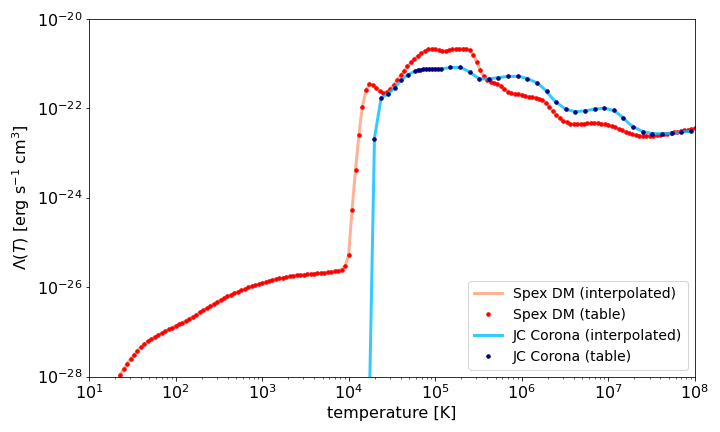
\includegraphics[width=\textwidth]{coolingcurves.png}
  \caption{
    Plots of two cooling curves $\HLFcool$ as a function of temperature. Red denotes the curve given by \citet{schure2009}, extended to low temperatures using \citet{dalgarno1972}. Blue denotes the curve given by \citet{colgan2008}. Dots represent values from the original tables, solid lines a local second-order polynomial approximation.
  }
  \label{fig: coolingcurves}
\end{figure}

Now, suppose a plasma that gains energy from an external source (constant heating in this case) and loses energy to its surroundings through optically thin radiative cooling processes (cooling), but is in full thermal equilibrium such that these two contributions cancel each other out (i.e. $\HLF_0 = 0$). This thermal equilibrium state will only be maintained if the plasma is stable with respect to small perturbations, such that any deviation from this state is counteracted and the plasma returns to its initial configuration.

Now assume that this plasma is at a certain uniform temperature at which $\dHLFT$ is negative, that is, the value of $\HLFcool$ increases when temperature decreases. This is the case at e.g. two million Kelvin (see Figure \ref{fig: coolingcurves}) for both cooling curves. If this plasma is perturbed such that the temperature decreases slightly, $\dHLFT < 0$ implies that the radiative losses will increase and the plasma loses even more energy, decreasing the temperature even further. This process will happen relatively slow at first, but after a while the plasma reaches a point of no return and a \emph{catastrophic cooling phase will kick in}: the small, initial perturbation that lowered the temperature grows and leads to \emph{thermal instability}. Nature's tendency is to keep pressure equilibrium, and according to the ideal gas law $p = \rho T$ the initial drop in temperature is accompanied by an increase in density in an (in this case futile) attempt to restore pressure balance. This has an adverse effect on the plasma as the heat-loss function $\HLF$ as defined here is dependent on density, meaning that a density increase leads to more energy losses. This, combined with the continuing drop in temperature leads to a runaway cooling process: the plasma density keeps increasing while the temperature keeps decreasing, giving rise to high-density, low-temperature regions.
A density perturbation can also give rise to thermal instability in the same manner as before: an increase in density implies a decrease in temperature or vice-versa (pressure balance), hence a temperature disturbance and the possibility to trigger instability. The effect of $\dHLFT$ on the growth rate of thermal instability is in general much stronger than $\dHLFrho$, except in regions where the heat-loss function has a relatively flat temperature dependence. In those cases the disturbance in density may actually be the dominant mechanism to trigger instability instead of temperature, where the density changes lead to cooling/heating variations.

The above discussion treats the case in which energy losses increase for decreasing temperature, but the reverse (i.e. $\dHLFT > 0$) may also give rise to instability. Here a drop in temperature decreases the energy losses, such that the heating term becomes dominant and heats up the plasma. A similar runaway process starts, where plasma density now decreases in an attempt to restore pressure equilibrium, lowering radiative losses even further. Generally speaking this process can also be referred to as ``thermal instability'', this time driven by heating. However, both cases give rise to both high density and low density plasma regions, such that we will not distinguish between the two.

Plasmas that are thermally stable will eventually return to thermal equilibrium after small perturbations. Due to the strong link between stability and $\dHLFT$, this will mainly happen in regions where the temperature dependence is minor, that is, for flat regions in the cooling curves. One such region may be just below $10^5$ K on Figure \ref{fig: coolingcurves}: here a small perturbation will only lead to a minor change in heating and cooling, such that the system has enough time to counteract the imbalance before the runaway reaction occurs. This may not be sufficient for perturbations that are large enough however, due to the delicate interplay between the heating and cooling terms, such that they might still be able to trigger instability.

If thermal conduction is also present then this will \emph{always} have a stabilising effect on the thermal instability. Initial temperature perturbations will be smoothened out due to thermal conduction effects, and even if the runaway cooling process has already started it will try and continue to do so. Generally speaking this stabilising behaviour will lead to a reduction of the thermal instability growth rate, but actually \emph{preventing} instability will only occur in a few select cases. The high anisotropy of thermal conduction plays a major role in magnetised plasmas as the effect is several orders of magnitude stronger parallel to the magnetic field lines than across, allowing for strong temperature gradients across field lines (and hence large $\dHLFT$ values). This implies that the direction of the wave vector is important, since perturbations more parallel to the magnetic field will be strongly stabilised, while wave vectors (near) perpendicular to the field lines will undergo almost no stabilisation by thermal conduction.

\begin{figure}[t]
  \centering
  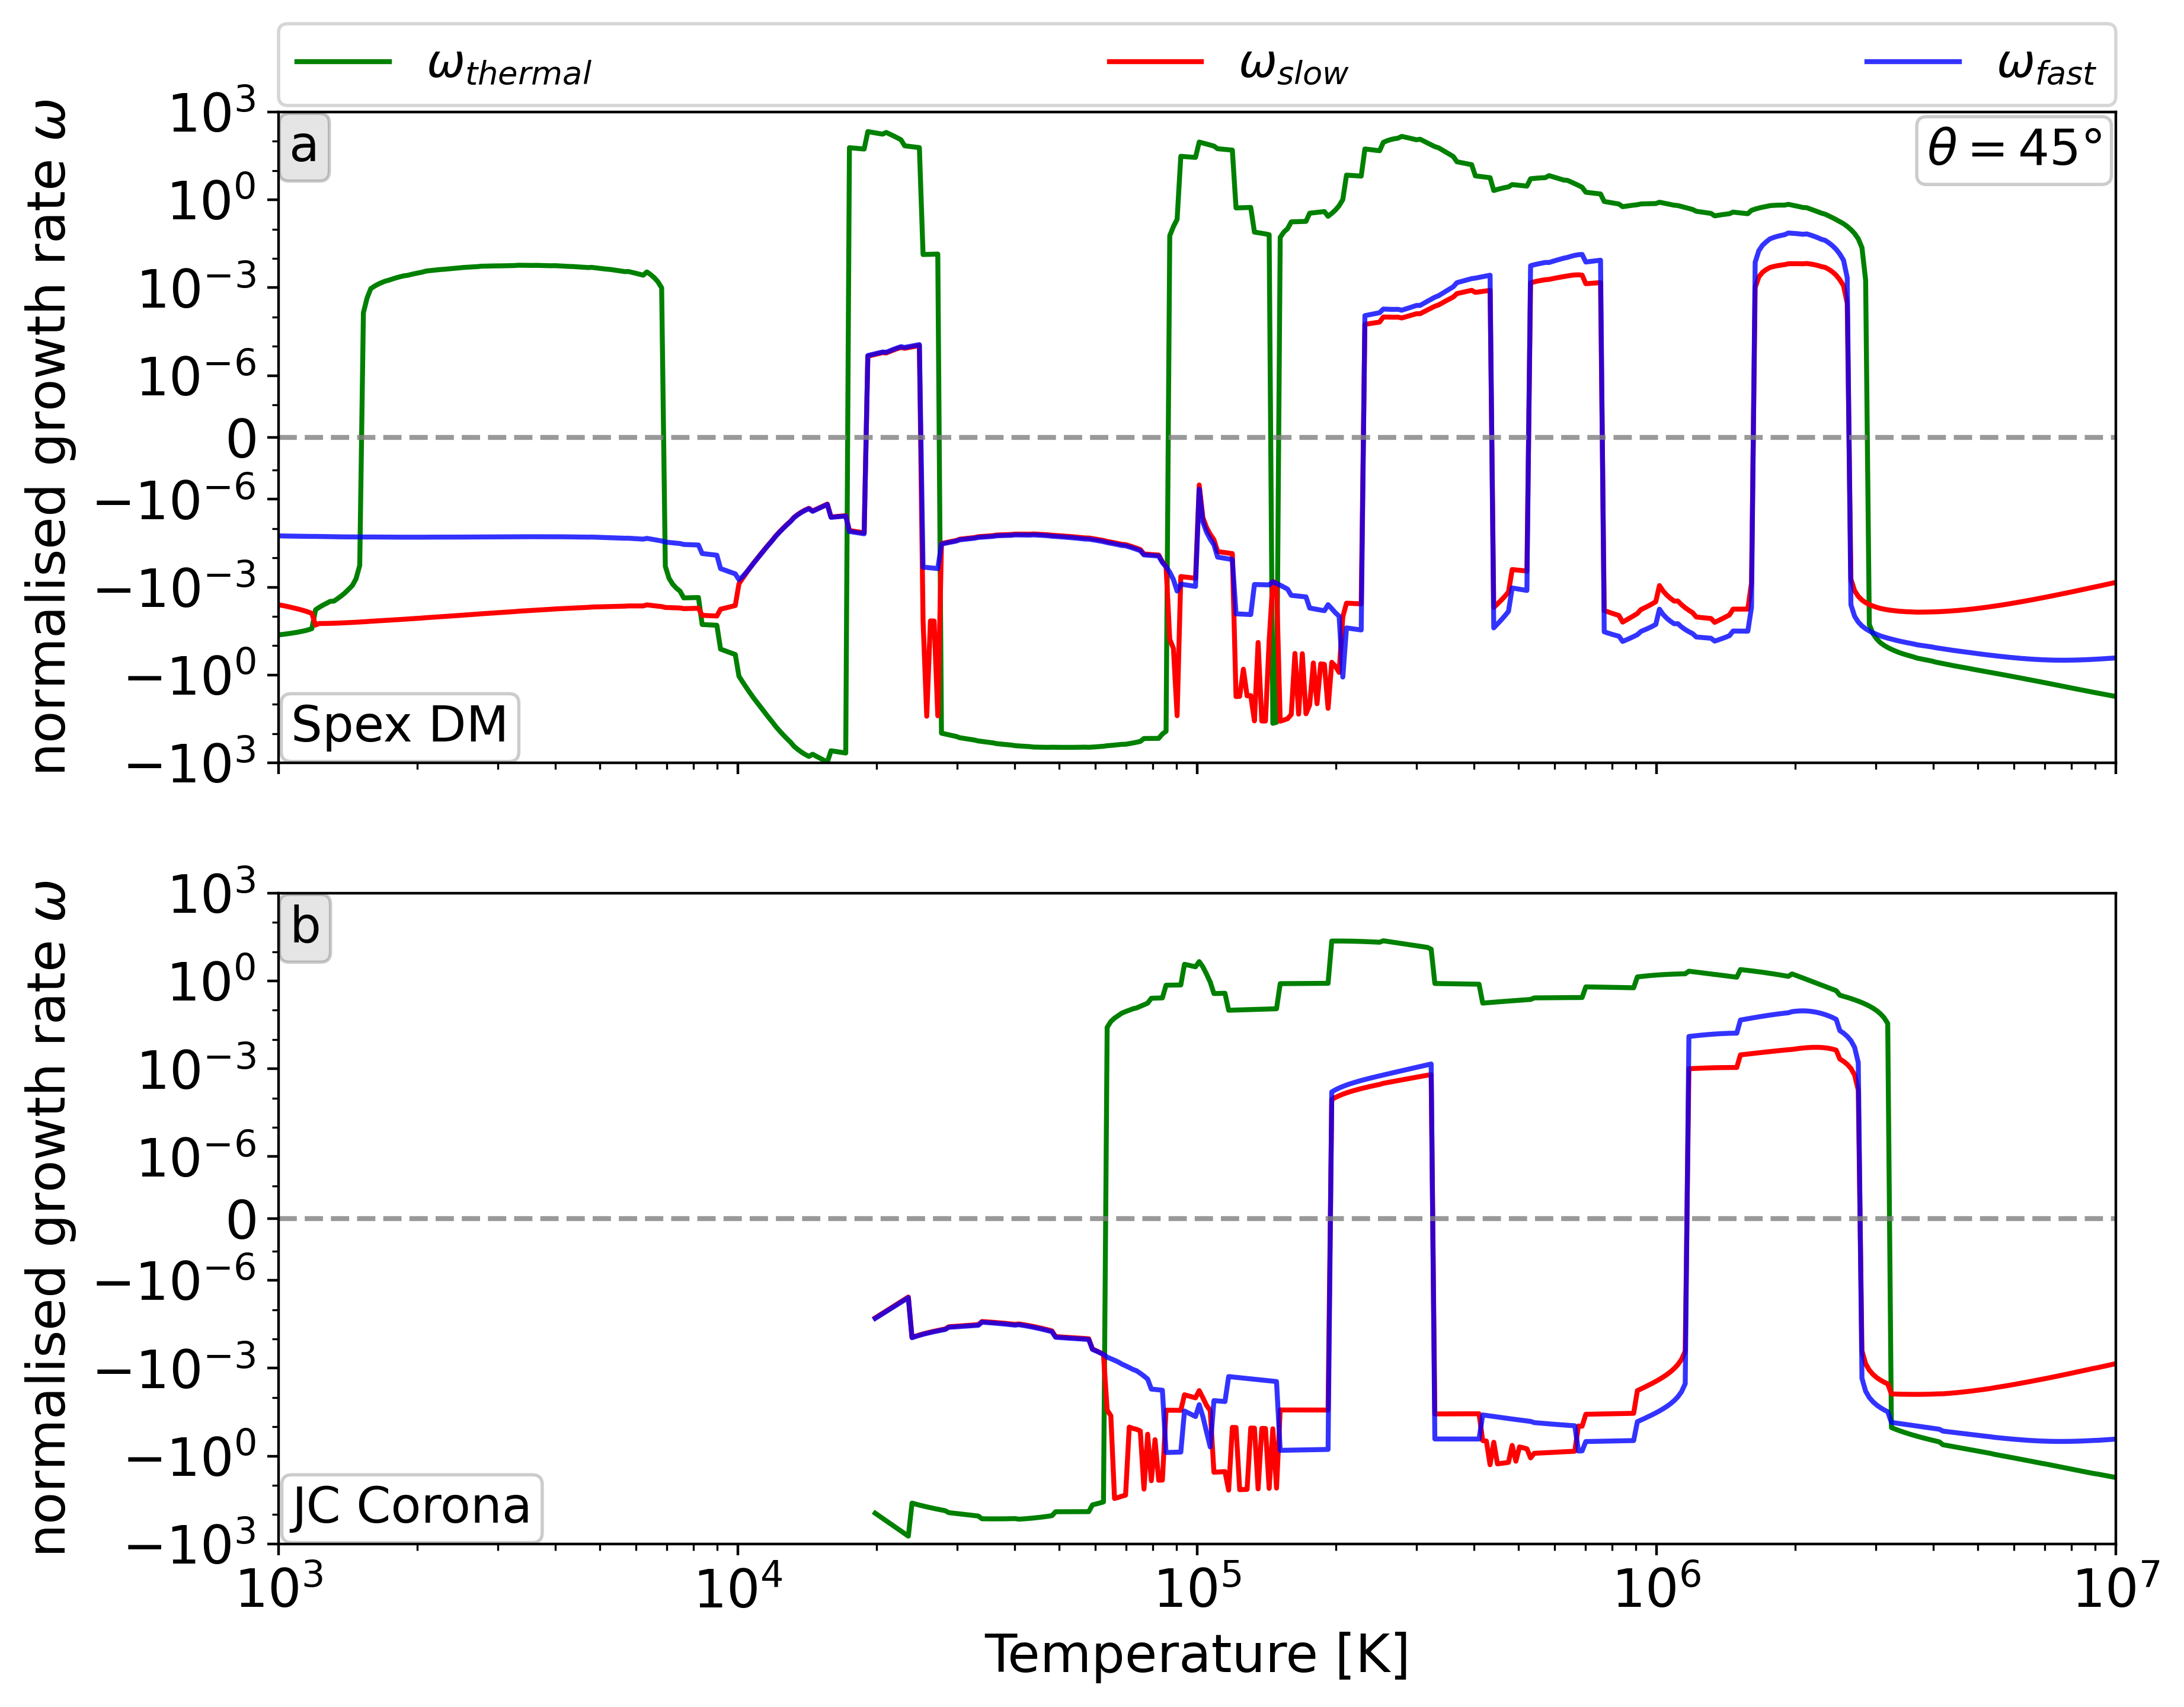
\includegraphics[width=\textwidth]{coolcurve_comparison.png}
  \caption{
    Normalised analytical growth rates $\omega_\text{I}$ as a function of temperature for the thermal (green), slow (red) and fast (blue) MHD modes, for an angle $\theta = \pi/4$ between the wave vector and magnetic field; thermal conduction and radiative cooling are included. Panel \textbf{a}: growth rates for the {\spexdm} cooling curve; Panel \textbf{b}: growth rates for the {\jccorona} cooling curve. Density is equal to unity (normalised), the uniform magnetic field is taken to be 10 Gauss.
  }
  \label{fig: coolcurve_comparison}
\end{figure}

Figure \ref{fig: coolcurve_comparison} shows a comparison between growth rates for the {\spexdm} (Panel a) and {\jccorona} (Panel b) cooling curves as a function of temperature. Radiative losses and thermal conduction are included; the angle between the wave vector $\bk$ and the uniform magnetic field $\bb_0$ is $\theta = \pi/4$. Overall mode stability, especially for the slow and fast modes, is quite dependent on the choice of cooling curve. The sharp cut-off near 20 000 K on Panel b is due to the {\jccorona} curve not having any tabulated values for lower temperatures (see Figure \ref{fig: coolingcurves}).

All of the above, which assumes a plasma at uniform temperature and a constant heating term, is ideal to get an intuitive feeling what thermal instability is and how it originates. In reality however things are much more complicated: the plasma is certainly not uniform, and in general the heat-loss function will have a complicated dependency on other (thermodynamic) variables. This implies that the process of thermal instability is much more intricate in fully realistic plasmas with regard to (in)stability, but the general idea holds: an unstable thermal mode triggers a runaway radiative cooling reaction, which in turn leads to high-density, low-temperature condensations.


\section{Thermal instability and nonlinear fragmentation}
As explained in the previous Section thermal instability leads to condensations. What we are now interested in is the spontaneous emergence of fine structure in these high-density condensations and how this evolves under typical solar coronal conditions. As mentioned in the introductory part of this Chapter both solar prominences and coronal rain condensations most likely originate from thermal instabilities in the solar corona, and it is still not understood how non-linear instability evolution shapes the observed fine structure of prominences. Investigating this requires multi-dimensional, high-resolution simulations to resolve all emerging substructure in great detail. This is what we embark upon for the remainder of this Chapter. However, first we have to know under which conditions thermal instabilities can actually form. We already discussed the intricate dependence of thermal stability on the heat-loss function, which in turn implies that we have both stable and unstable regions. For this we need detailed knowledge of the growth rates of the various modes, which we can obtain by solving the eigenvalue problem. Once we have identified these regions of interest we can setup our numerical simulations.


\subsection{Eigenfunctions}
Before diving into the simulation aspect of this Chapter we first change the background orientation of the magnetic field vector and wave vector. We plan to perform numerical simulations of a given setup and the usual convention is to align the magnetic field itself with one of the coordinate axes -- just as we have been doing up to now. Here we will do the opposite: aligning the wave vector $\bk$ with the $x$-axis while the magnetic field $\bb_0$ will be aligned in the 3D coordinate system. The advantage of this is that we can use periodic boundary conditions on all sides of the domain in our numerical simulations. If we would have kept the general convention as-is then all waves would propagate at some arbitrary angle with respect to the coordinate axes, such that it would have been quite difficult to make use of periodic boundary conditions, even more so when imposing multiple waves on top of each other. We can therefore define $\bk$ and $\bb_0$ as follows
\begin{equation}
  \bk = (k_x, 0, 0), \qquad\qquad \bb_0 = \left(B_{0x}, B_{0y}, B_{0z}\right).
\end{equation}
Using this convention we can rewrite the system of linear MHD equations \eqref{eq: linearised_rho1_homo}-\eqref{eq: linearised_A1_homo} in terms of the unknown variables. This results in the eigenfunctions associated with a specific orientation of the wave vector $\bk$ with respect to the magnetic field $\bb_0$, given by
\begin{gather}
  \rho_1 = \frac{k_x \rho_0}{\omega}v_{1x}, \label{eq: rho1_eigenfunction}\\
  v_{1y} = \frac{B_{0x}B_{0y}k_x^2}{B_{0x}^2k_x^2 - \omega^2\rho_0}v_{1x}, \\
  v_{1z} = \frac{B_{0x}B_{0z}k_x^2}{B_{0x}^2k_x^2 - \omega^2\rho_0}v_{1x}, \\
  T_1 = -\frac{k_x \rho_0 \gmone \left(\icomplex\dHLFrho\rho_0 - T_0 \omega\right)}{
    \omega\left[
      \icomplex\gmone\left(\kappapara\kpara^2 + \kappaperp\kperp^2\right)
      + \icomplex\gmone \dHLFT \rho_0
      + \omega \rho_0
    \right]
  }v_{1x}, \\
  A_{1y} = \frac{\icomplex B_{0z}\omega \rho_0}{B_{0x}^2k_x^2 - \omega^2\rho_0}v_{1x}, \\
  A_{1z} = -\frac{\icomplex B_{0y}\omega \rho_0}{B_{0x}^2k_x^2 - \omega^2\rho_0}v_{1x}, \label{eq: A1Z_eigenfunction}
\end{gather}
where the eigenfunctions for the $x$-component of the vector potential $A_{1x} = 0$. All of the above eigenfunctions have a dependence on $v_{1x}$, such that this eigenfunction can be chosen arbitrarily. Similar results can be obtained when $\bk$ is aligned along a different coordinate axis or when shifting to 2D. The main advantage of having the actual eigenfunctions is that we can now consistently excite a specific MHD wave mode associated with a certain eigenvalue $\omega$ in numerical simulations. The eigenfrequency itself can be obtained by solving the eigenvalue problem just as we did before.

\subsection{Numerical setup}
To perform the simulations we make use of the parallelised Adaptive Mesh Refinement Versatile Advection Code MPI-AMRVAC \citep{keppens2012_amrvac,porth2014_amrvac,xia2018_amrvac} to numerically solve the full non-linear, non-adiabatic MHD equations on a two- or three-dimensional Cartesian mesh with multiple levels of adaptive mesh refinement (AMR). The base resolution used in all simulations is $100^2$ and $100^3$ for the 2D and 3D results, respectively. Three (3D) and five (2D) levels of AMR are used with the trigger of refinement based on a density criterion, achieving a maximum effective resolution of $400^3$ and $1600^2$ near high-density regions in 3D and 2D, respectively. As indicated further, one ultra-high resolution run in 2D uses seven AMR levels for a $6400^2$ run to reveal more details. The length scale of the system is of the order of a few to 10 Mm depending on the simulation. In MPI-AMRVAC both the radiative cooling contribution and conduction effects are handled as additional source terms to the energy equation. {\spexdm} is used as a cooling curve, the heating term is taken to be constant over time and equal to the radiative losses at $t = 0$, implying that the radiative losses and heating contribution balance each other at $t = 0$ such that an initial state of thermal equilibrium is achieved. Thermal conduction is treated in full tensorial form, a detailed explanation on how the code handles conduction effects parallel and perpendicular to the magnetic field is provided in \citet{xia2018_amrvac}.

\subsubsection{Initial conditions}
We use periodic boundary conditions on all sides of the domain and start from a uniform thermal equilibrium state as described before. The wave vector $\bk$ is always equal to $2\pi$ divided by the domain length to ensure one single oscillation along one of the axes to satisfy the periodic boundary conditions on all sides (in other words, the wave ``fits'' nicely in the domain). The magnetic field orientation with respect to the coordinate axes is described by an angle $\theta$, measured from the $xy$-plane towards the $z$-axis, and by an angle $\delta$ measured in the $xy$-plane from the $x$-axis towards the $y$-axis. Using this description the background magnetic field $\bb_0$ can be written as
\begin{equation}
  \bb_0 = \left(B_0\cos\theta\cos\delta, B_0\cos\theta\sin\delta, B_0\sin\theta\right).
\end{equation}
In two dimensions the expression for $\bb_0$ becomes straightforward, as we only have a single angle $\theta$ between $\bb_0$ and $\bk$. However, in three dimensions there is possible ambiguity when talking about wave vector components ``parallel'' and ``perpendicular'' to the magnetic field lines, and as such we defined these as
\begin{equation}
  k_{x, \parallel} = \frac{\cos\theta}{\cos\delta}k_x
  \qquad \text{and} \qquad
  k_{x, \perp} = \frac{\sin\theta}{\cos\delta}k_x,
\end{equation}
for a wave vector $\bk$ aligned with the $x$-axis. As initial perturbations we use the eigenfunctions as given in Equations \eqref{eq: rho1_eigenfunction}-\eqref{eq: A1Z_eigenfunction}. For simulations without thermal conduction the coefficients $\kappapara$ and $\kappaperp$ can be set to zero.

We initialise all simulations using slow MHD waves, that is, taking the eigenvalue corresponding to the slow mode solution of the eigenvalue problem and using that to initialise the eigenfunctions.
For the initial perturbation $v_{1x}$ we take a plane wave given by
\begin{equation} \label{eq: vx_sims}
  v_{1x} = C\Bigl[\cos(k_x x) + \icomplex \sin(k_x x)\Bigr],
\end{equation}
where $C$ is some constant amplitude taken to be $10^{-3}$. Similar expressions can be used when $\bk$ is aligned along a different axis, for example along the $y$-axis all eigenfunctions become dependent on $v_{1y}$ which can again be taken arbitrarily and similar to Equation \eqref{eq: vx_sims}. Unless explicitly stated otherwise all equilibrium configurations considered in this Chapter have a density of $\rho_n = 2.34 \times 10^{-15}$ g cm$^{-3}$ (a standard coronal value) and a magnetic field strength of $B_0 = 10$ Gauss. This field value is typical for prominences \citep{gibson2018}. The pressure in all simulations is calculated using the ideal gas law, following $p = \rho T$ in normalised units. The combination of periodic boundary conditions on all sides and a conservative numerical scheme ensures that the total mass across the domain is conserved at all times, such that any condensation is thus an in situ process where mass gets redistributed but not created or destroyed. This is unlike evaporation-condensation configurations such as in \citet{xia2016}, where mass accumulates in the corona from evaporating chromospheric matter.

\subsubsection{Magnetic field treatment}
When one is doing calculations in MHD it is always possible to make sure that the divergence-free condition on the magnetic field $\nabla \cdot \bb = 0$ is satisfied analytically. However, it is far from trivial to fulfil this requirement in simulations, as floating-point precision, round-off errors and numerical approximations may introduce a small divergence of the magnetic field. This deviation from zero can in turn grow over time, and if one is not careful to properly account for this the results may become unphysical. Various methods have been developed to tackle this problem, such as adding sources proportional to numerical monopole errors to balance them out or doing parabolic cleaning to diffuse any local error compliant with the limits of the time step. In our simulations we use the \textsf{constrained transport} feature of MPI-AMRVAC, which was first implemented and demonstrated in its general relativistic MHD code variant BHAC \citep{porth2017_bhac}. This method ensures that if the initial magnetic field, staggered on cell face centres, is integrated from a vector potential on the cell edges then the initial magnetic field divergence at cell centres is zero up to machine precision in a particular discretisation. Hence, we initialised the vector potential on cell edges for the initial equilibrium state, as is implemented in the code. We can therefore define $\ba_0$ for the background equilibrium as
\begin{equation} \label{eq: homo_vectorpotential}
  \ba_0 = \left(B_{0y}z, B_{0z}x, B_{0x}y\right).
\end{equation}
This retrieves the original homogeneous $\bb_0$ when calculating $\bb_0 = \nabla \times \ba_0$, and the real part of the perturbations (i.e. eigenfunctions) in the vector potential are consequently added to the above expressions.

\subsection{Thermal stability regions}
Before fixing all equilibrium conditions, that is, choosing a temperature value and a particular magnetic field orientation, we have to pay special attention to the actual stability and instability regimes of the thermal mode in the presence of thermal conduction. As discussed before the latter always has a stabilising effect on thermal instability since temperature variations are rapidly smoothed out by field-aligned thermal conduction. However, we can always quantify the critical wave number $\kcrit$, which in essence implies that perturbations with a wave number above $\kcrit$ (or equivalently, with a small enough wavelength) are completely stabilised by thermal conduction. This critical wave number can be derived by doing a stability analysis on the corresponding dispersion relation, however, we will not do that here and instead refer to the thorough derivation given by \citet{field1965}. By changing the length scale of our numerical domain, we effectively change the wave number in the direction that the perturbation is applied, while still keeping a single oscillation to satisfy the periodic boundary conditions. In taking a longer wavelength, we are able to excite an unstable thermal mode even with the inclusion of thermal conduction. Thermal instability itself is not triggered if the homogeneous equilibrium configuration is stable to the thermal mode.

\begin{figure}[t]
  \centering
  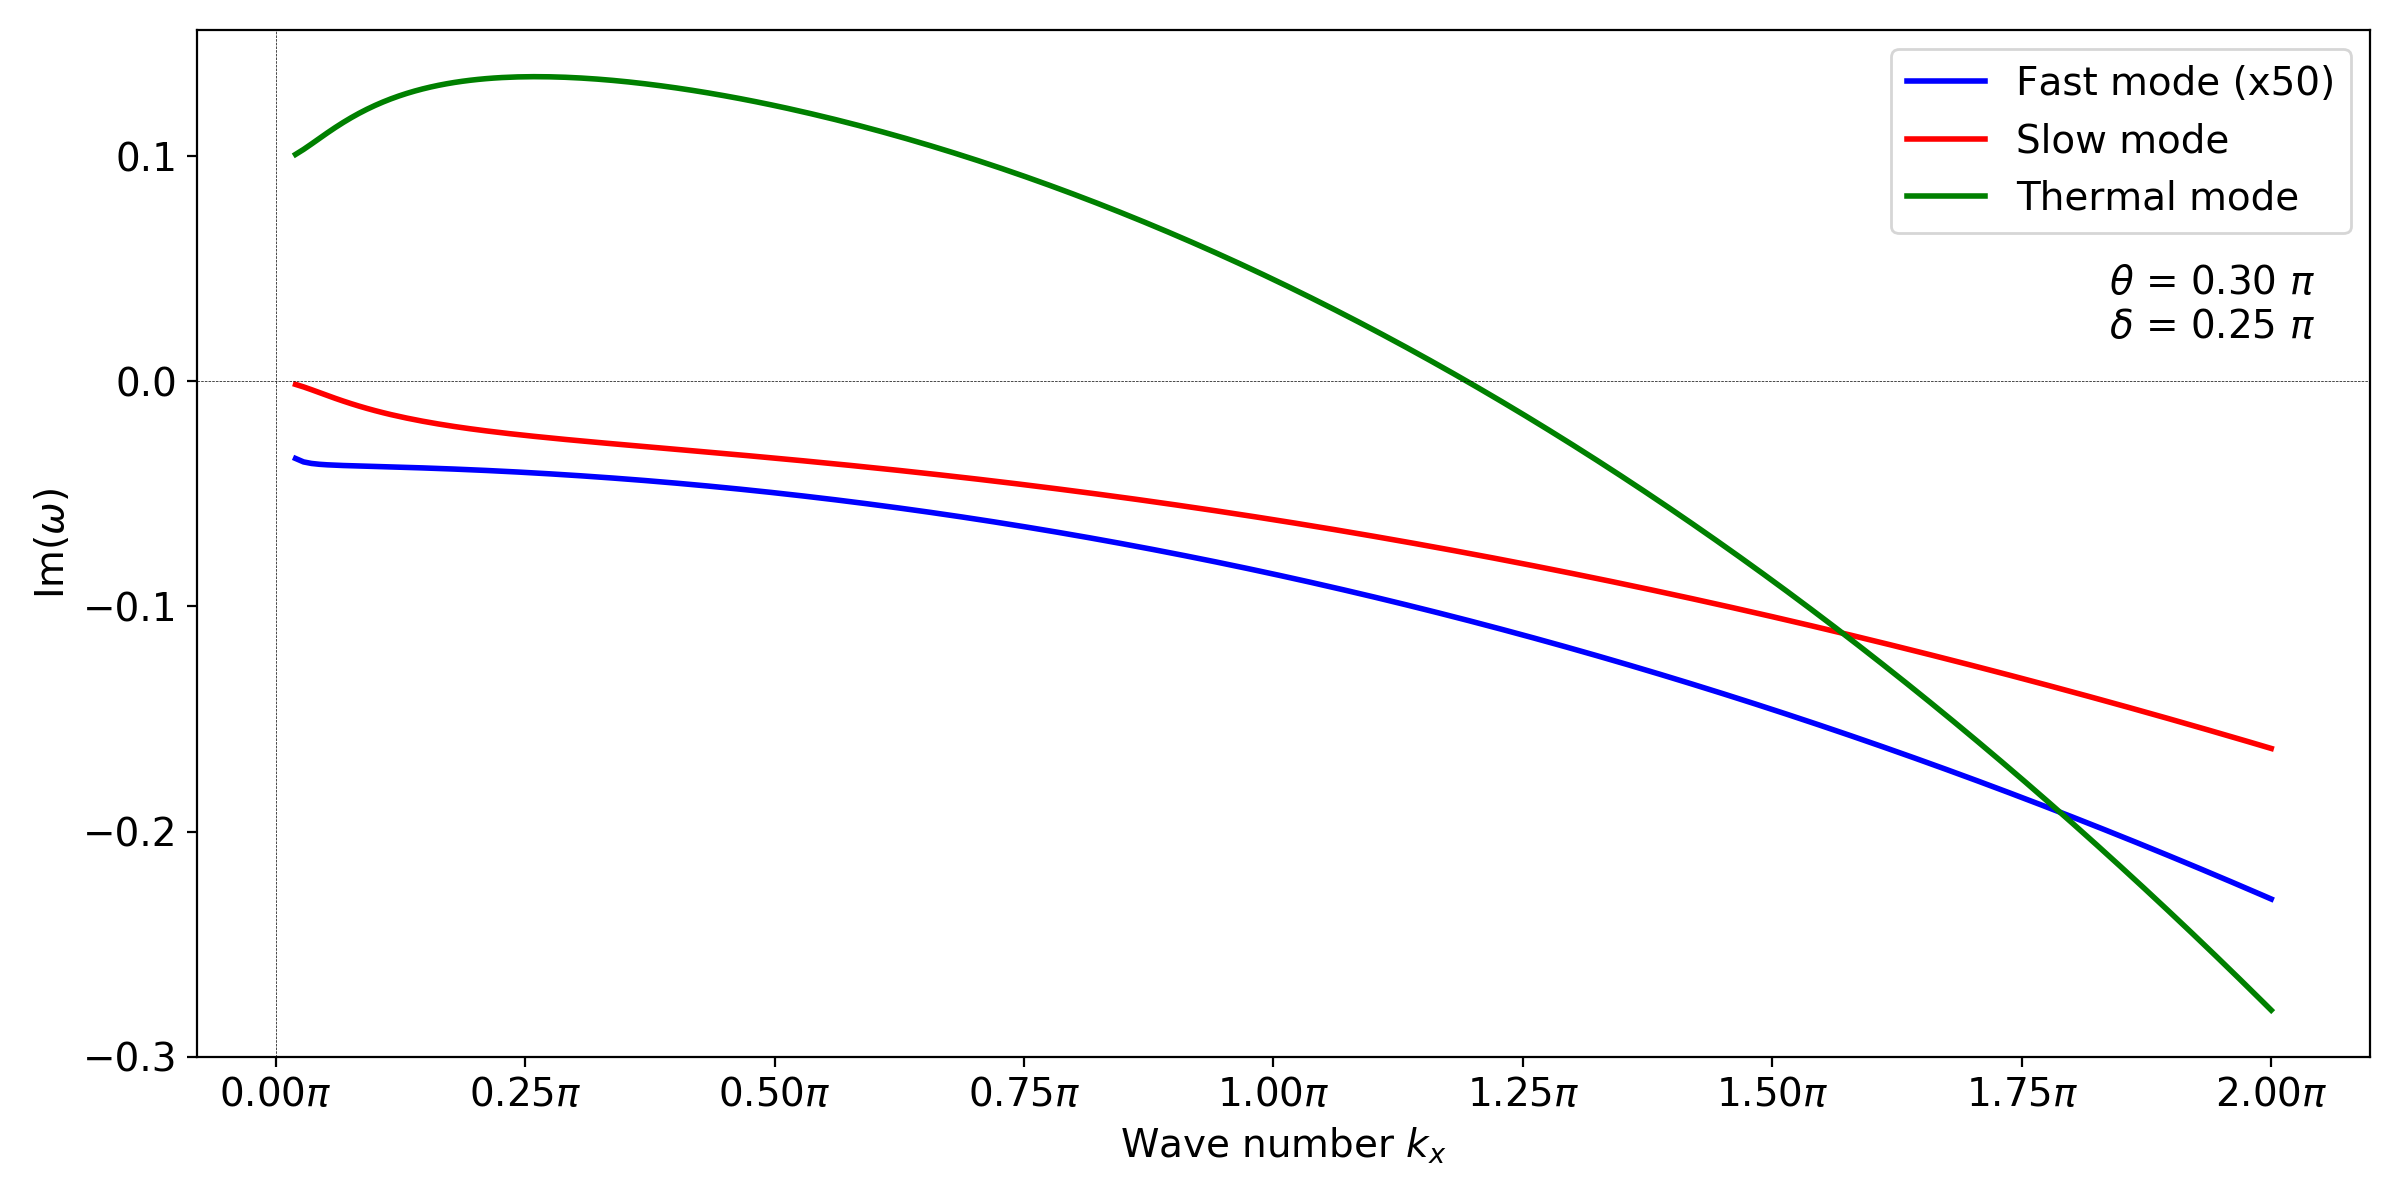
\includegraphics[width=\textwidth]{w_vs_kx.png}
  \caption{
    Analytical growth rates of the MHD modes as a function of wave number, for $\bk$ aligned with the $x$-axis for an angle $\theta = 0.3\pi$ and $\delta = \pi/4$. The thermal mode is stable above $k_x \approx 1.2\pi$, which is the critical wave number for these conditions. The growth rate of the fast mode was multiplied by 50 for clarity. The equilibrium temperature is 0.5 MK; the density and magnetic field are the default values.
  }
  \label{fig: w_vs_kx}
\end{figure}

Figure \ref{fig: w_vs_kx} shows the analytical growth rate of all three relevant modes under typical solar coronal conditions, where we now fix the temperature to 0.5 MK and a given field orientation; the growth rates are shown as a function of wave number. The wave vector $\bk$ was taken along the $x$-axis. The slow and fast wave modes are damped everywhere under these conditions, but the thermal mode shifts from stability to instability when going below the critical wave number. The angles $\theta$ and $\delta$ were given a value of $0.3\pi$ and $\pi/4$, respectively. Note that all growth rates are specified in normalised units, with a unit time equal to $t_0 \approx 85.87$ seconds.

\begin{figure}[t]
  \centering
  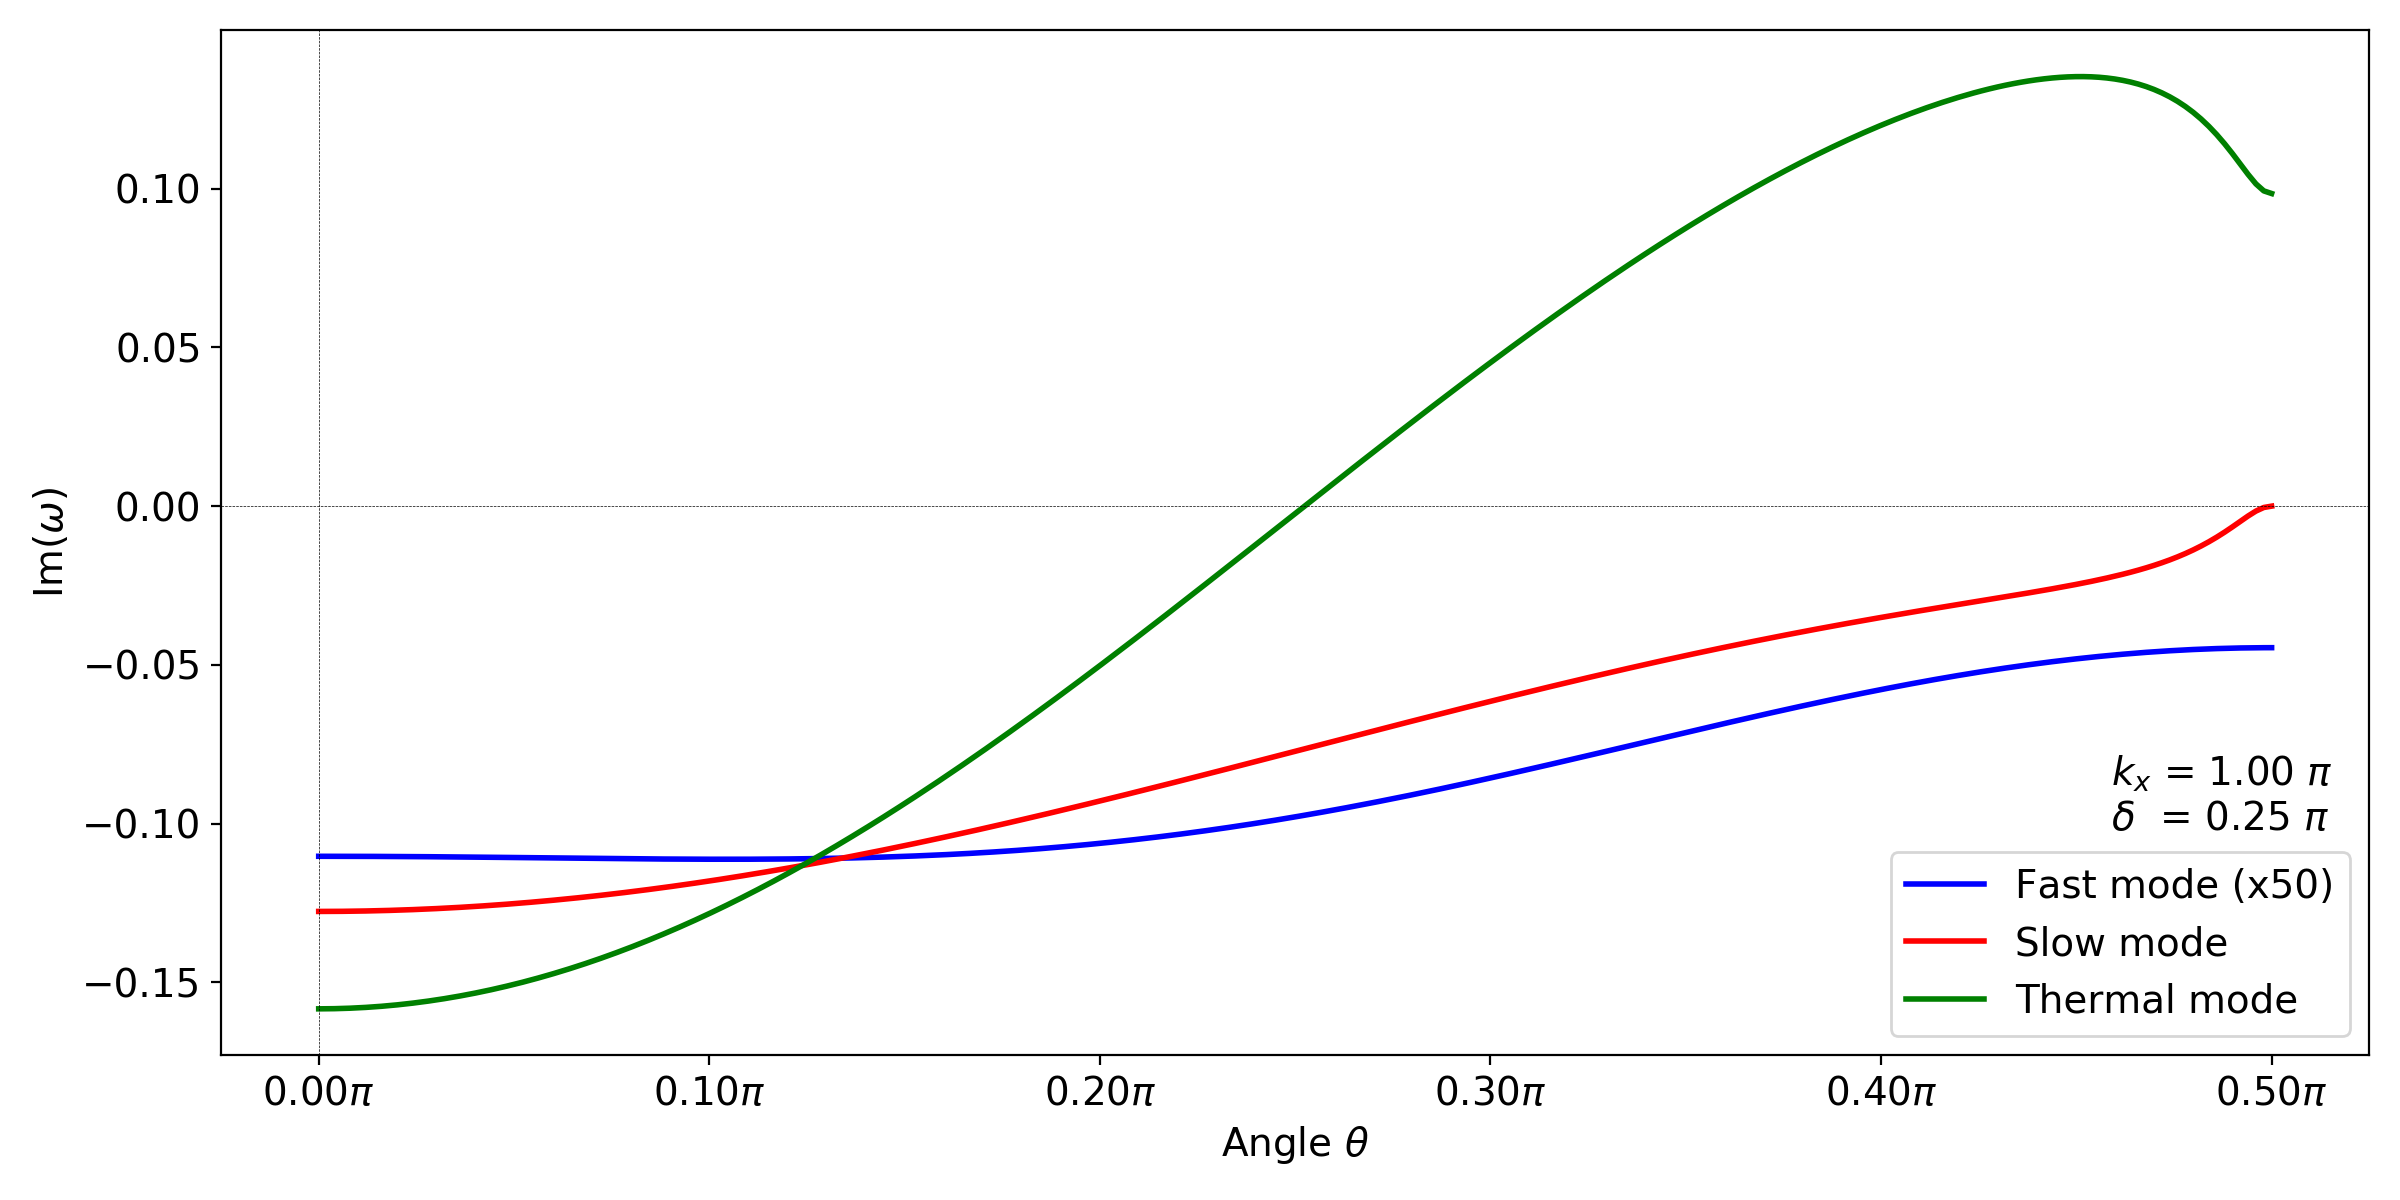
\includegraphics[width=\textwidth]{w_vs_theta.png}
  \caption{
    Analytical growth rates of the MHD modes as a function of $\theta$ for a fixed value of $\delta = \pi/4$ and $k_x = \pi$. The wave vector $\bk$ is aligned with the $x$-axis. The thermal mode becomes unstable for $\theta > \pi/4$, at this point parallel thermal conduction is too ineffective for stabilisation to occur due to the alignment between $\bb_0$ and $\bk$. The growth rate of the fast mode was multiplied by 50 for clarity. The equilibrium temperature is 0.5 MK; the density and magnetic field are the default values.
  }
  \label{fig: w_vs_theta}
\end{figure}

Figure \ref{fig: w_vs_theta} on the other hand indicates that solely considering the critical wave number is not sufficient for instability of the thermal mode. The wave number was taken to be $k_x = \pi$, which according to Figure \ref{fig: w_vs_kx} should indicate instability. However, when the angle $\theta$ is varied and becomes too small (for a fixed $\delta = \pi/4$) the magnetic field becomes too aligned with the wave vector such that the contribution of parallel thermal conduction is particularly effective in smoothing out emerging temperature variations. Only for values of $\theta > \pi/4$ does thermal conduction parallel to the field lines become inefficient enough, and consequently enables the thermal mode to become unstable under these conditions. Armed with this knowledge, all simulations we perform further on achieve conditions where the slow modes are damped, but the thermal mode is inherently unstable.


\subsection{Thermal instability onset in 2D}
To start we consider a purely 2D setup where we superimpose two slow MHD modes, one along each axis. This is done by calculating the eigenvalues and eigenfunctions for each $\bk$, i.e. one along the $x$-axis and one along the $y$-axis, and exciting them in a similar way as described before. These waves interact with each other, but are both damped owing to the slow-mode stability in Figures \ref{fig: w_vs_kx} and \ref{fig: w_vs_theta} (the growth rates $\omega_\text{I}$ are negative). Because we excited the eigenfunctions in a regime that is unstable to the thermal mode, this regime eventually becomes excited and takes over as soon as the waves are sufficiently damped out. The thermal mode starts to grow, locally increasing the density, leading to an increased cooling contribution and a lower temperature. This eventually results in high-density, low-temperature filaments, and it is important to stress that the term ``filament'' in this context does not specifically refer to the solar feature, but rather to a simple high-density, low-temperature region.

\begin{figure}[t]
  \centering
  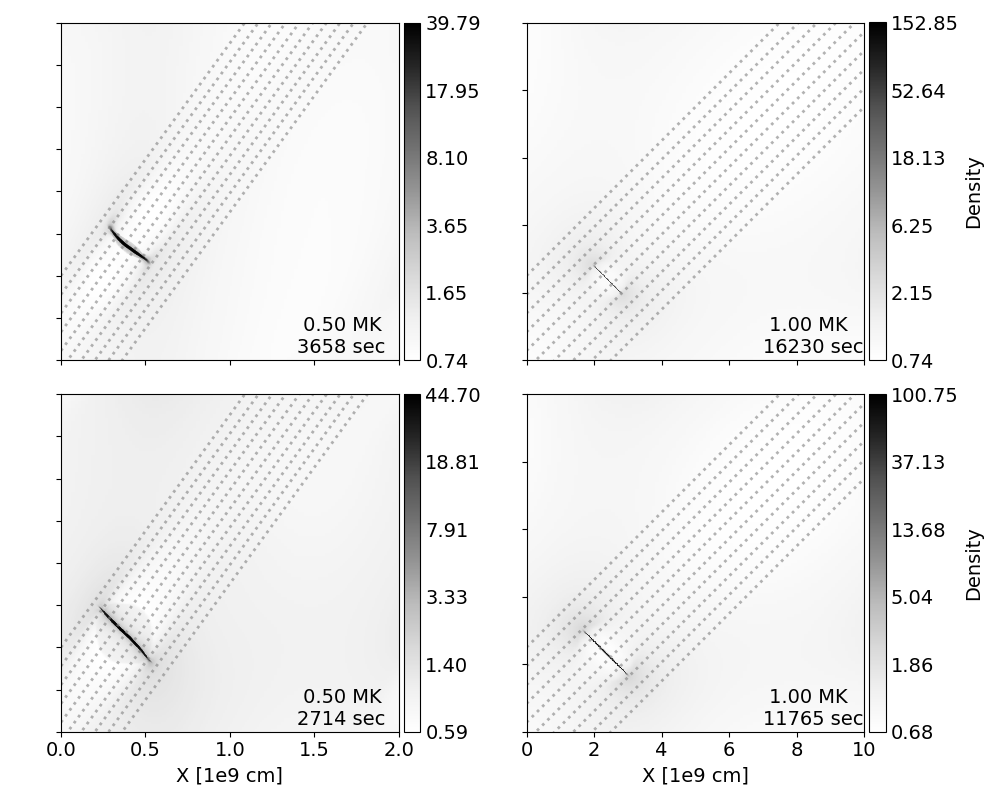
\includegraphics[width=0.9\textwidth]{2d_instability_onsets.png}
  \caption{
    Density view at the onset of thermal instability for a background temperature of 0.5 MK (\emph{left column}) and
    1 MK (\emph{right column}), with conduction (\emph{top rows}) and without conduction (\emph{bottom rows}). The formation of the high-density filament happens approximately perpendicular to the magnetic field lines, annotated with dotted lines, in all cases. The density is normalised to $\rho_n$
  }
  \label{fig: 2d_instability_onsets}
\end{figure}

Figure \ref{fig: 2d_instability_onsets} shows the onset of TI, just after the high-density filament is formed but before the breaking-up phase. Two equilibrium temperatures are considered, 0.5 MK in the left column and 1 MK in the right column, thermal conduction is included for the top row and omitted for the bottom row. Because of the stabilising effect of thermal conduction, the onset of TI occurs at a later time than without conduction (due to smaller growth rates); the actual physical times are denoted on the figure panels. The magnetic field lines are superimposed using dotted lines on each panel and make an angle $\theta = 0.3\pi$ and $\theta = 0.25\pi$ with the $x$-axis for the left and right columns, respectively. It should be noted that the right two panels of Figure \ref{fig: 2d_instability_onsets} have a larger domain size because the thermal mode is less unstable at one million Kelvin. We thus needed to adjust the box size to ensure that the wavelength of the system becomes larger and $|\bk|$ smaller, satisfying the critical wave number criterion for instability.

\subsubsection{Ram pressure and filament fragmentation}
The onset of filament formation depicted in Figure \ref{fig: 2d_instability_onsets} indicates that in all cases the high-density filament seems to form nearly perpendicular to the magnetic field, such that material is literally flowing towards the high-density region along the field lines. This effect in turn creates a velocity difference on opposite sides of the filament, consisting of two counter-streaming flows of matter and a high-density region in-between.

\begin{figure}[t]
  \centering
  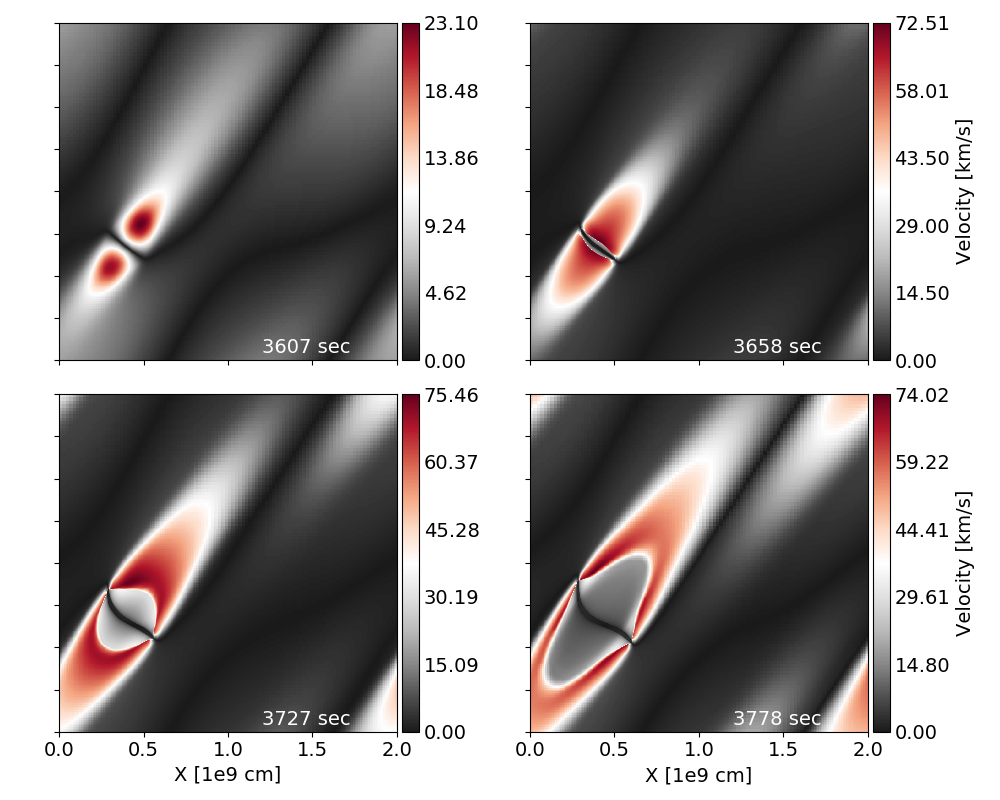
\includegraphics[width=0.8\textwidth]{2d_velocity_plots.png}
  \caption{
    Velocity magnitude for the simulation corresponding to the top left panel of Figure \ref{fig: 2d_instability_onsets} but with more AMR levels. The first collision of low-pressure induced flows along the field lines produces a rebound slow shock on either side of the filament, travelling outwards.
  }
  \label{fig: 2d_velocity_plots}
\end{figure}

In order to investigate this effect in greater detail we chose one of the simulations shown above, namely the 0.5 MK case with thermal conduction, increased the number of AMR levels to seven and let it run far into the non-linear regime, long after the filament has formed. This increase in refinement achieves a maximum effective resolution of $6400 \times 6400$, corresponding to a smallest cell size of 3.125 km. Since the typical length scale of coronal rain is on the order of a few 100 km, any occurrence of small high-density blobs in the far-nonlinear regime are resolved. All figures mentioned in this subsection correspond to this particular simulation.



Figure \ref{fig: 2d_velocity_plots} shows a detailed view of the formation process of the high-density region, at four different snapshots. The magnitude of the velocity field is shown, starting at the onset of filament formation. There is clearly a large velocity difference on either side of the high-density region owing to the infalling matter on a trajectory aligned with the magnetic field. The filament itself appears mostly stationary, representing an in-situ formation process. It is enclosed by an outwards moving shock front on both sides. The slow and Alfv\'en wave velocities can be roughly estimated near to the shocked region, yielding $\approx 60-70$ km s$^{-1}$ and $\approx 400$ km s$^{-1}$, respectively, such that we are dealing with slow MHD shocks enclosing the filament. These findings are in line with previous results obtained in \citet{xia2012} and \citet{fang2015}, where this rebound shock phenomenon was also encountered in their simulations on prominence formation and coronal rain, respectively.

\begin{figure}[t]
  \centering
  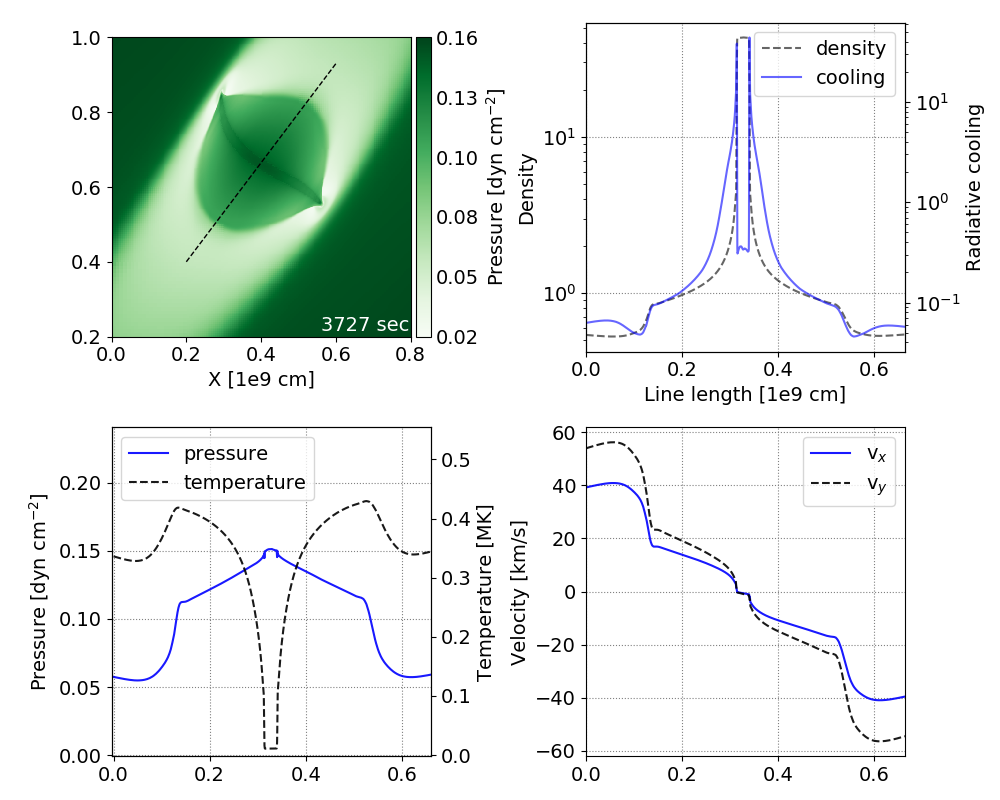
\includegraphics[width=\textwidth]{2d_lineplots.png}
  \caption{
    Pressure view (\emph{top left panel}) along with various physical quantities along the indicated line, crossing the high-density blob. Density is normalised to $\rho_n$.
  }
  \label{fig: 2d_lineplots}
\end{figure}

Figure \ref{fig: 2d_lineplots} shows a plot of the different physical quantities over a line spanning the high-density blob and the shock fronts. The top left panel shows a zoomed-in view of the pressure, with the selected line indicated in black. Density and radiative cooling jump about two orders of magnitude when crossing the blob. Both gas pressure and temperature show a considerable increase over the shock fronts due to the compression and shock heating of the plasma, the blob itself is at a temperature of approximately 10 000 K. The bottom right panel shows the velocity components over the selected line, dropping almost to zero inside the blob, indicating a near stationary state. Sharp increases again denote the shock front itself, impacting the higher-velocity inflowing plasma.

The fourth panel of Figure \ref{fig: 2d_velocity_plots} shows a later stage, in which the shocks have propagated even further and start to fan out. These rebound shocks are generated at the same time as the formation of the high-density region and are caused by the first collision of low-pressure induced inflows of matter. After the filament has formed the inflows fall into the transition region between the condensation and shock fronts, without generating new shocks. This effect in turn feeds matter to the filament, causing it to extend further. The shock fronts sweep up and shock-heat matter when travelling outwards; their propagation speed is mostly determined by the gradually matter-evacuated environment of the filament. This implies faster shock propagation perpendicular to the filament (parallel to the magnetic field), and slower propagation perpendicular to the field lines (parallel to the filament). This in turn causes a pinching effect related to the ram pressure, as the ends of the filaments are pinched between the outer edges of the rebound shocks. This is an inherently unstable configuration in which any small velocity difference on either side causes the filament to stretch out and undergo a torque. This effect is also clearly visible on the fourth panel of Figure \ref{fig: 2d_velocity_plots}.

The pinching phenomenon becomes very clear when looking at the ram pressure surrounding the system. Since we are dealing with two opposite velocity vectors, but parallel to the magnetic field, we can assume that the original inflow is approximately perpendicular to the filament surface, and later to the shock fronts. In this case the expression for the ram pressure can be roughly simplified to the density multiplied by the square of the velocity magnitude. Figure \ref{fig: 2d_ram_pressure} shows the ram pressure at four different snapshots, with the first one at the same time as the fourth panel on Figure \ref{fig: 2d_velocity_plots}. Here the pinching effect is clearly visible, but, more importantly, there is an asymmetry present between ram pressures on either side of the filament ends. This becomes even more clear on the second panel in which the ram pressure on the bottom side of the right end is much higher than on the opposite side, and the same (but in reverse) holds for the left side of the filament. This effect stretches out the filament and redistributes it across the domain. However, at this point the original filament is thinned out by all the stretching, such that certain regions are particularly susceptible to small imbalances in the velocity or pressure. This is exactly what is happening on the fourth panel of Figure \ref{fig: 2d_ram_pressure}, which shows a zoomed-in view of a part of the filament, indicated by the enclosing box. Small blobs start to form, driven by small imbalances in ram pressure, which cause fragmentation of the filament. This kind of phenomenon is typical for a thin-shell instability, first described in \citet{vishniac1983}.

\begin{figure}[t]
  \centering
  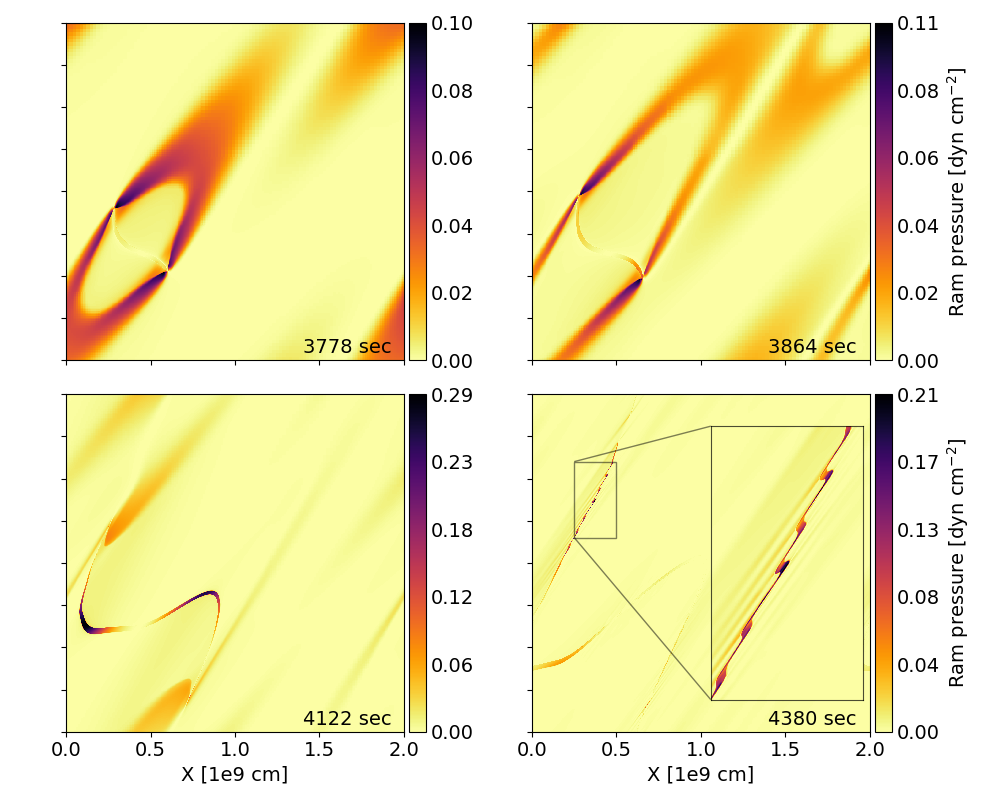
\includegraphics[width=\textwidth]{2d_ram_pressure.png}
  \caption{
    Ram pressure at four different snapshots after filament formation. The first panel corresponds to the fourth panel in Figure \ref{fig: 2d_velocity_plots}. The sequence clearly shows how ram pressure is responsible for the stretching (top right and bottom panels) of the filament. The inset on the fourth panel is a zoom-in on part of the filament, where small ram pressure imbalances cause instabilities and fragmentation through the thin-shell instability.
  }
  \label{fig: 2d_ram_pressure}
\end{figure}

Figure \ref{fig: 2d_density_fragmentation} shows the density evolution right after filament formation, all the way up to the fragmentation process. The rebound shocks are visible on the first panel, the second panel shows how the filament is stretched out owing to ram pressure differences. Fragmentation starts to occur on the third panel near to the outer ends of the filament through the thin-shell instability. In the fourth panel there is even more fragmentation, where now even the central filament region is breaking up. The inset zooms in on one of the fragmenting regions, the smallest blobs have a width of the order of a few tens of grid cells (at the highest resolution), corresponding to a physical length scale of a few 100 km, consistent with typical coronal rain sizes.

\begin{figure}[t]
  \centering
  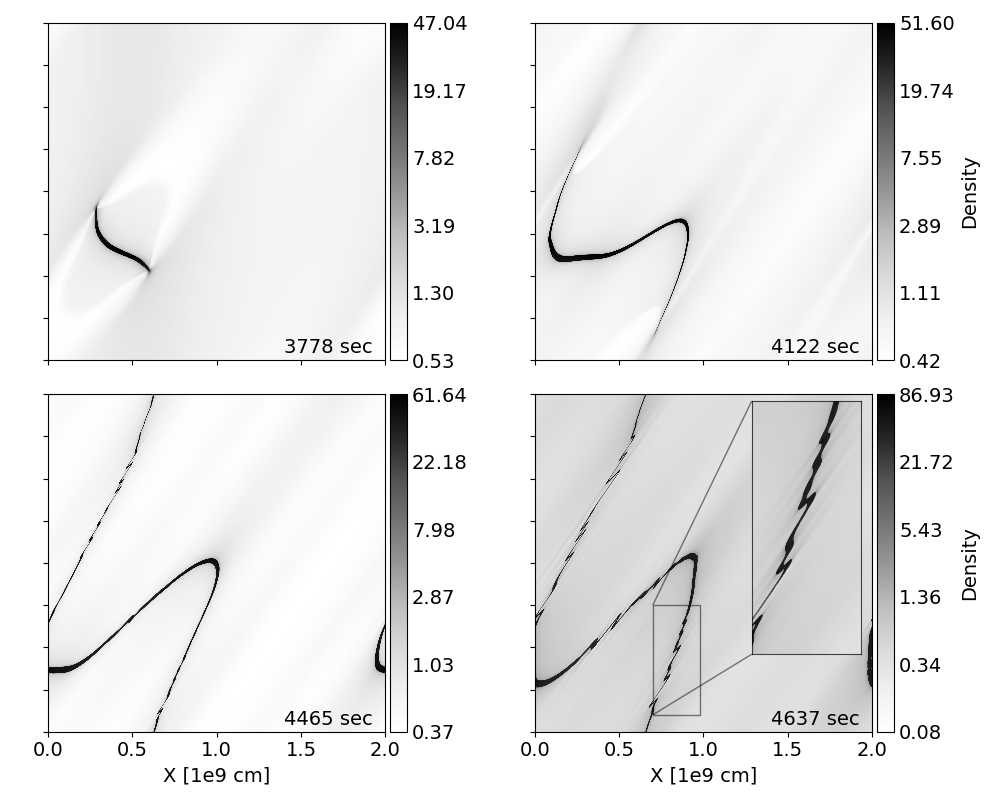
\includegraphics[width=\textwidth]{2d_density_fragmentation.png}
  \caption{
    Density plots right after filament formation (first panel) and far into the nonlinear regime (other panels). The filament starts to fragment on the third panel through the thin-shell instability. Fragmentation has progressed even further in the last panel, where the inset zooms in on one of the regions that are breaking up into smaller blobs. Density is normalised to $\rho_n$.
  }
  \label{fig: 2d_density_fragmentation}
\end{figure}


\subsection{Thermal instability onset in 3D}
Next we look at how the above translates to a 3D setup in which three slow waves are superimposed, again taken along the coordinate axes. All slow modes are damped but the configuration is unstable to the thermal mode, hence the entire process towards TI is similar as in 2D: the waves interact with each other and damped out, but due to thermal instability a runaway cooling reaction is triggered and a high-density region forms.

\begin{figure}[t]
  \begin{minipage}{0.45\textwidth}
    \centering
    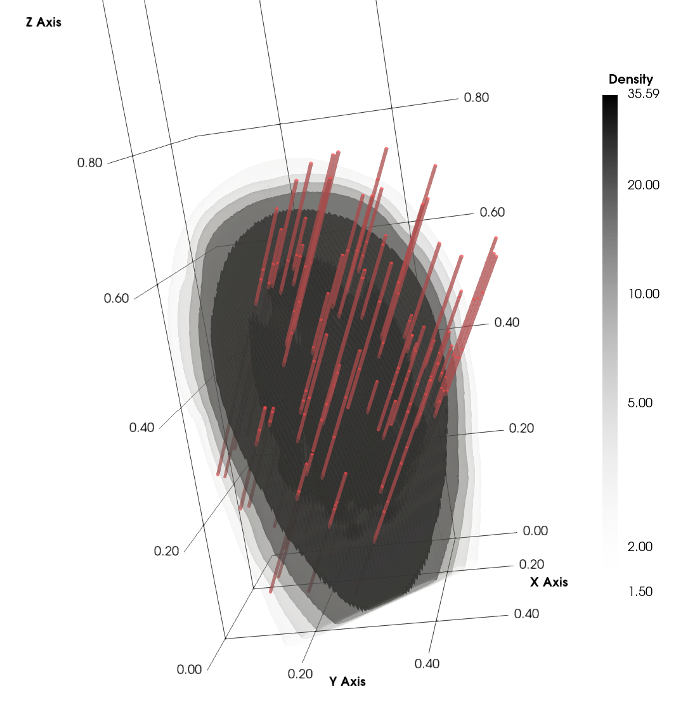
\includegraphics[width=\textwidth]{3d_instability_onset.png}
  \end{minipage}
  \begin{minipage}{0.54\textwidth}
    \centering
    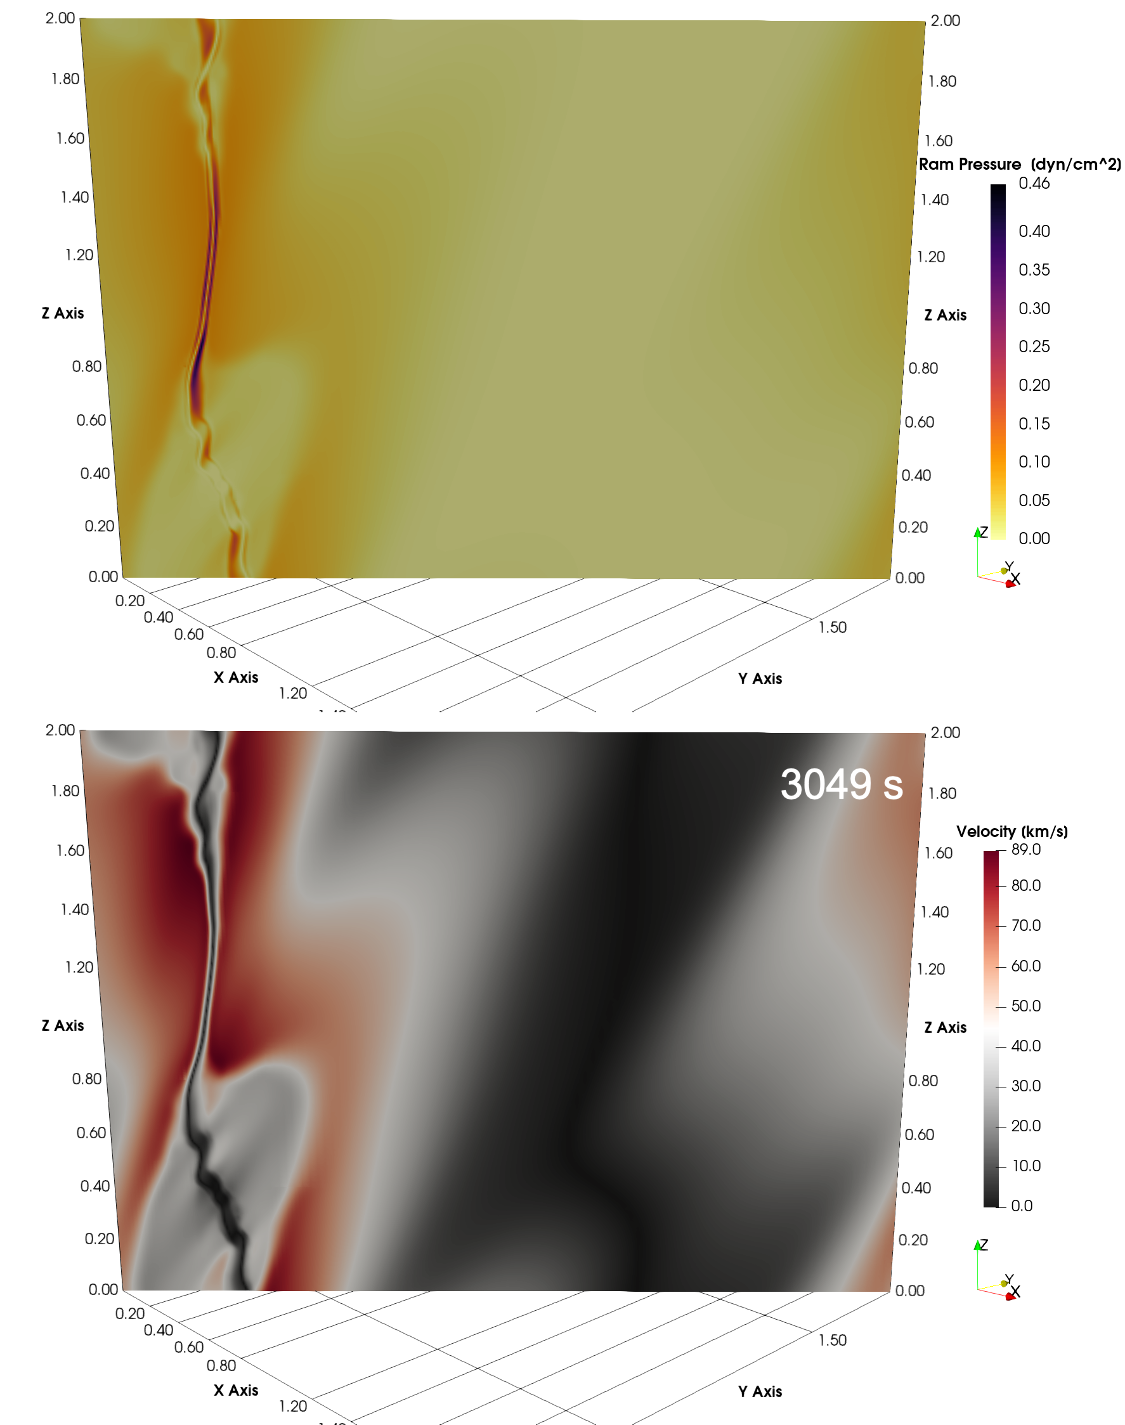
\includegraphics[width=\textwidth]{3d_pressure_velocity.png}
  \end{minipage}
  \caption{
    \textbf{Left}: Density isocontours at the onset of filament formation in three dimensions. Magnetic field lines are shown in red. Density is normalised to $\rho_n$, the snapshot is taken at approximately 2920 seconds. This is the onset of thermal instability; no fine structure is yet present. \textbf{Right}: slices showing ram pressure (\textbf{top}) and velocity magnitude (\textbf{bottom}) at $t \approx 0.85$ h. Two outwards travelling rebound shocks are present which fan out over time. Kinks in the filament and ram pressure differences on opposite sides denote the onset of thin-shell instability, fragmenting the high-density region.}
  \label{fig: 3d_onset_pressure_velocity}
\end{figure}

The left side of Figure \ref{fig: 3d_onset_pressure_velocity} shows the onset of the high-density region in three dimensions for the same equilibrium parameters as the 0.5 MK simulation in 2D (Figures \ref{fig: 2d_velocity_plots} -- \ref{fig: 2d_density_fragmentation}). The only exception is that in this case the magnetic field has a different alignment due to the 3D setup, making an angle $\theta = 0.3\pi$ and $\delta=\pi/4$. Density isocontours are shown, and similar to the 2D case the formation of the high-density region appears to occur almost perpendicular to the magnetic field lines, which are drawn in red on the figure. The right side of this figure depicts slices diagonally taken across the 3D domain, parallel to the $z$-axis, showing the ram pressure distribution and velocity magnitude. Various regions of higher ram pressure surround the filament, alternated by lower ram pressure voids. Similar to the 2D case, outwards travelling rebound shocks can be seen that sweep up and shock heat the plasma. The actual pressure and velocity values in these regions are comparable to the 2D results and are again slow wave shocks. The pinching effect caused by the expanding shock fronts is again present, albeit less pronounced than for the 2D case discussed before.

\begin{figure}[t]
  \centering
  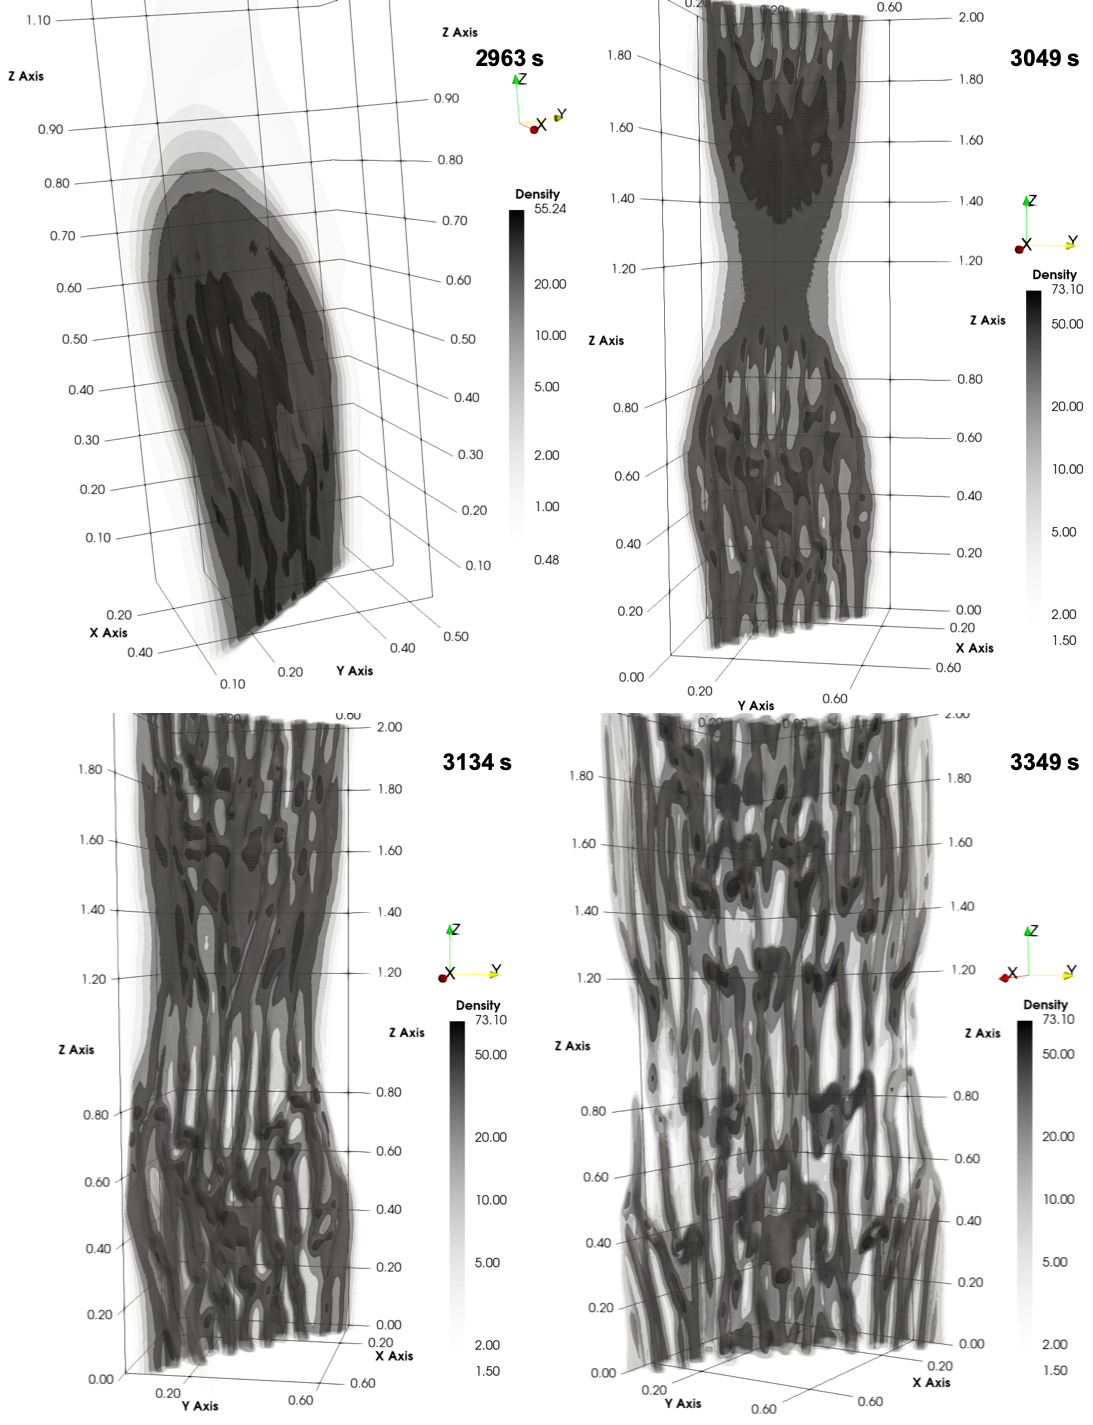
\includegraphics[width=0.62\textwidth]{3d_density_evolution.png}
  \caption{
    Density isocontours at four different snapshots in the 3D simulations, the physical time is denoted on each panel. The filament has fragmented and appears to coalesce into multiple dense blobs, interconnected by various higher-density strands, forming a morphologically complex web of fine structure.
  }
  \label{fig: 3d_density_evolution}
\end{figure}

Figure \ref{fig: 3d_density_evolution} shows density isocontours of different snapshots, where the top right panel corresponds to the same time as the diagonal slices in Figure \ref{fig: 3d_onset_pressure_velocity}. Two major differences between the 2D and 3D cases should be noted. First, because of periodic boundary conditions the bottom part of the filament re-enters the domain at the top as shown in the first two panels of Figure \ref{fig: 3d_density_evolution}. However, this has no major influence on the substructure itself, as fragmentation and the formation of elongated strands occurs before this happens. The first panel of Figure \ref{fig: 3d_density_evolution} already shows slightly higher density regions and some weak filamentary substructure which become even more distinct on the second panel, and by the time the third panel is reached the process results in one large high-density region spanning the entire $z$-axis of the domain, showing a very complex morphology. On the last panel, the higher density regions have coalesced into blobs, interconnected by a web of slightly less dense, elongated strands.

\begin{figure}[t]
  \centering
  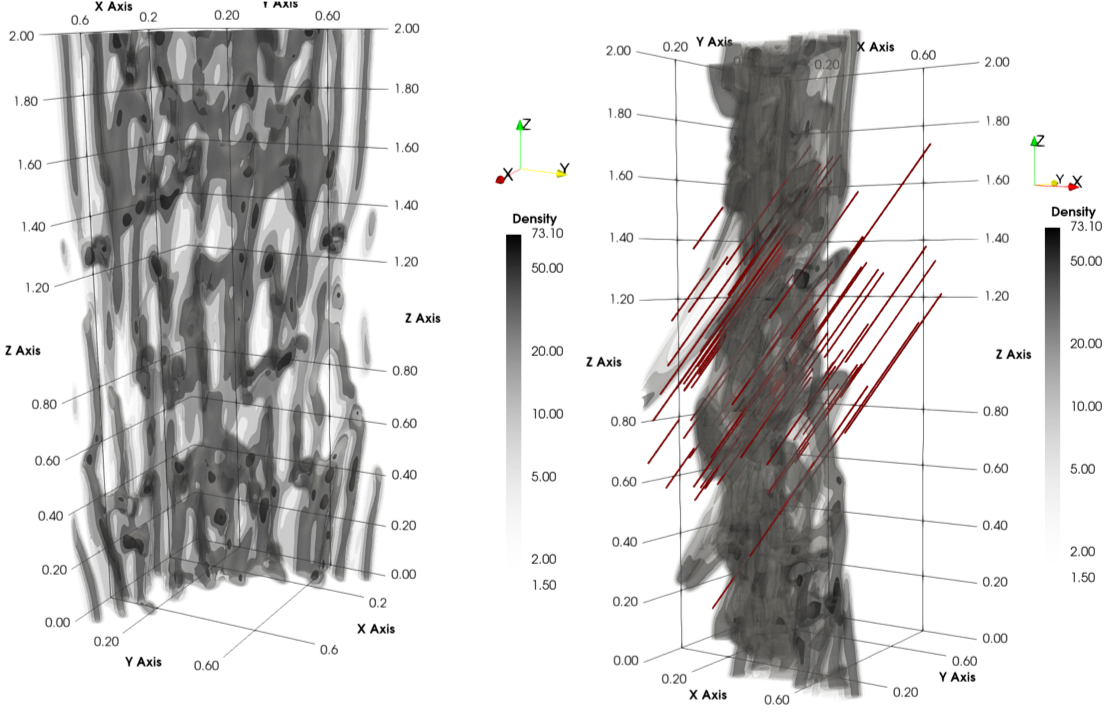
\includegraphics[width=0.8\textwidth]{3d_density_final.png}
  \caption{
    Density isocontours at approximately 3365 seconds. The left and right panels represent different viewing angles, the magnetic field lines rare denoted in red.
  }
  \label{fig: 3d_density_final}
\end{figure}

The second difference to discuss is the alignment between the high density threads and the background magnetic field. Figure \ref{fig: 3d_density_final} shows the final snapshot of the 3D simulation for two different viewing angles, with the right panel rotated about 90 degrees counterclockwise around the $z$-axis with respect to the left panel; the magnetic field lines are drawn in red. On the left the overall picture is not so different from the last panel in Figure \ref{fig: 3d_density_evolution}, except that some long strands have broken op into multiple, smaller ``blob''-like pieces with high density. What should be noted however is that these strands are not at all aligned with the magnetic field lines. We see that some blobs appear to move outwards, away from the main high density region, guided by the magnetic field. This implies that the actual condensation is \emph{aware} of the magnetic field orientation, but is not necessarily completely \emph{aligned} with it.

\begin{figure}[t]
  \begin{minipage}{0.5\textwidth}
    \centering
    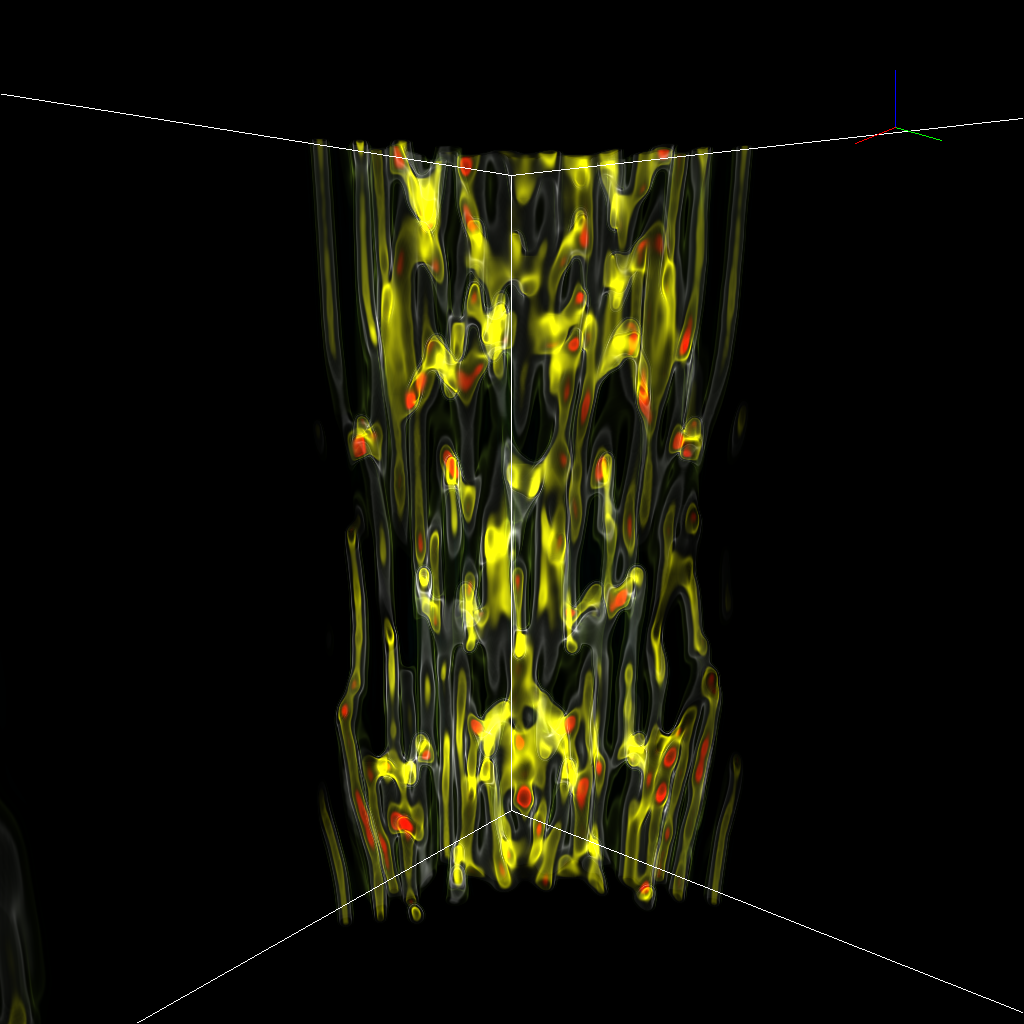
\includegraphics[width=\textwidth]{3d_volume_rendering.png}
  \end{minipage}
  \begin{minipage}{0.49\textwidth}
    \centering
    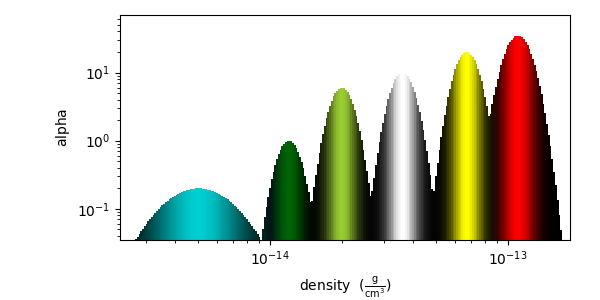
\includegraphics[width=\textwidth]{3d_transfer_function.png}
  \end{minipage}
  \caption{
    \textbf{Left}: volume rendering of the filamentary fine structure at approximately 3564 seconds (last snapshot).
    \textbf{Right}: a custom transfer function, tweaked to highlight high density regions. The solid white lines denote the domain boundaries. This rendering was made by \textsf{yt} \citep{turk2011} using the MPI-AMRVAC frontend.
  }
  \label{fig: 3d_volume_rendering}
\end{figure}

This last conclusion becomes very clear when looking at a volume rendering of the high density filaments in figure \ref{fig: 3d_volume_rendering}. The transfer function was customised and tweaked for high densities such that dense regions appear orange-red, while less dense regions have a more green-blue colour. The transfer function itself is shown on the right panel, where the alpha value is shown as a function of density. The red and yellow Gaussians are centred at $1.1 \times 10^{-13}$ and $6.7 \times 10^{-14}$ g cm$^{-3}$, respectively, with high alpha values to make these regions stand out. The Gaussians denoting the light green and white colours are centred at $2 \times 10^{-14}$ and $3.6 \times 10^{-14}$ g cm$^{-3}$, respectively, with an approximately similar alpha value. The darker green and blueish parts of the transfer function have their centres at $1.2 \times 10^{-14}$ and $5 \times 10^{-15}$ g cm$^{-3}$, respectively, where the alpha values were significantly lowered as to reduce the contribution of the ambient medium, which would otherwise completely blur the image. In this rendering the multi-stranded nature of the main high-density regions becomes very clear, where the elongated threads are shown in a yellowish colour embedded in slightly less dense strands, with the denser, cool blobs appearing in red. The final snapshot of the simulation is shown, where we see some blobs moving away from the high density region in a direction that appears to be guided by the magnetic field lines.

\subsubsection{Synthetic views}
To stress the emerging fine structure and field misalignment even further, we created synthetic $\halpha$ views of the 3D simulation discussed above using a method described by \citet{heinzel2015}. First, the ionisation degree $\alpha_\text{i} = n_\text{e}/n_\text{H}$ and the parameter $f(T, p)$ -- which gives a relation between the electron density and hydrogen second-level population -- are interpolated at each grid point from pre-computed tables using the local thermal pressure and temperature. The $\halpha$ line absorption coefficient $\kappa_\nu$ is then given by
\begin{equation}
  \kappa_\nu = \frac{\pi e^2}{\masse c}f_{23}n_2 \phi_\nu(\nu),
\end{equation}
where $\masse$, $c$ and $n_2$ denote the electron mass, speed of light and hydrogen second-level population, respectively. The latter can be found through
\begin{equation}
  n_2 = \frac{n_\text{e}^2}{f(T, p)}
  \qquad \text{where} \qquad
  n_\text{e} = \frac{p}{\left(1 + \frac{1.1}{\alpha_\text{i}}\right)\boltzmanncte T}.
\end{equation}
The $\halpha$ line oscillator strength is given by $f_{23}$ and is approximately equal to 0.6407 \citep{goldwire1968}, $\boltzmanncte$ denotes the Boltzmann constant. For the absorption line profile we adopted a Gaussian function
$\phi_\nu(\nu)$ with a microturbulent velocity of 5 km s$^{-1}$. The optical thickness $\tau_\nu$ is then obtained by integrating along the line of sight (los), that is,
\begin{equation}
  \tau_\nu = \int_{\text{los}}\kappa_\nu(\nu, l)dl.
\end{equation}
This is then plugged into the radiative transfer equation $I(\nu) = S(1 - \exp(-\tau_\nu))$ assuming a uniform source function $S$, which is taken to be equal to the diluted $\halpha$ line-centre intensity at the solar disc centre, eventually yielding the $\halpha$ line intensity along a given line of sight.

Figure \ref{fig: 3d_synthetic_views} shows synthetic $\halpha$ views obtained by integration along the three coordinate axes for three different snapshots. Especially on the third column of panels, corresponding to the last snapshot in the simulation and Figure \ref{fig: 3d_volume_rendering}, the complex morphology of the filament threads and high-density blobs is clearly visible. The line-of-sight integration along the $z$-axis clearly shows the magnetic field awareness, aligned diagonally from the bottom left to the top right corner when projected onto the $xy$-plane ($\delta = \pi/4$).

\begin{figure}[t]
  \centering
  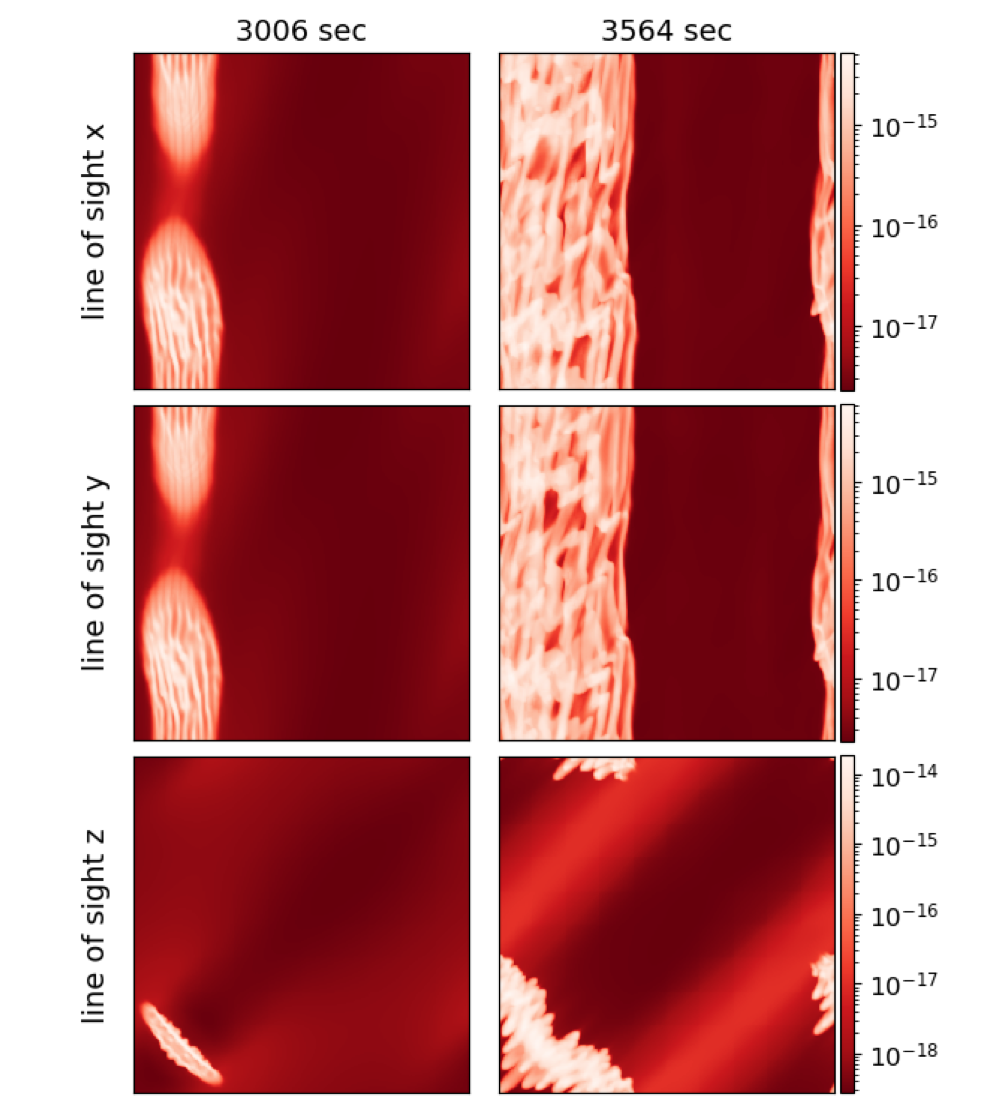
\includegraphics[width=0.8\textwidth]{3d_synthetic_views.png}
  \caption{
    Synthetic $\halpha$ views from the 3D simulation in Figure \ref{fig: 3d_density_evolution} for line-of-sight integrations along the three coordinate axes (\textbf{rows}) for two different snapshots (\textbf{columns}). The resulting projection further stresses the complex morphology of emerging fine structure; the bottom row of panels clearly shows the awareness of $\bb_0$, aligned diagonally when projected onto the $xy$-plane.
  }
  \label{fig: 3d_synthetic_views}
\end{figure}

The actual implications of these last findings are hence twofold. Firstly, the fact that fine structure can be aligned quite differently with respect to the magnetic field orientation directly extends to solar prominences and prominence substructure, implying that direct observation of fine structure alignment does not necessarily constrain the direction of the magnetic field. Secondly, these simulations were performed using a uniform equilibrium state, but can resemble local solar coronal conditions. This is especially relevant for the multi-stranded shape of solar prominences, since in the simulations discussed in this Chapter these features seem to occur in a natural way through a combination of thermal instability, thermal conduction effects, rebound shocks, and ram pressure differences. These latter two give rise to thin-shell instability; a pinching effect is caused by the outwards propagating shock fronts which elongates, turns and fragments the filament (2D), or through an early occurrence of ram pressure imbalances, immediately fragmenting the high density region before it can undergo a torque (3D). In both cases slow rebound shocks fan outwards, after which we eventually see fragmentation of the filament with high-density blobs guided by the magnetic field lines and fine structure not at all aligned with the background magnetic field.


\section{Discussion and implications}
It has been widely assumed that the orientation of filament fine structure can give some indirect information on the magnetic field topology in solar prominences. To that end this Chapter was dedicated to numerical 2D and 3D simulations of interacting slow waves with the inclusion of radiative cooling effects and anisotropical thermal conduction; the main findings can be summarised in a few key points:
\begin{enumerate}
  \item[i)] In order for thermal instability to trigger, the local plasma conditions must correspond to a regime unstable to the thermal mode. Both slow and fast waves are damped for solar conditions and in order for the thermal mode to be unstable in the presence of anisotropic thermal conduction the critical wavelength has to be satisfied. In any situation in which that is not the case, all modes dampen out.
  \item[ii)] When TI occurs the high density region appears to form orthogonal to the magnetic field lines, both in 2D and 3D. Material flows towards the filament following the magnetic field lines, guided by the strong pressure gradient. The first collision of low-pressure induced inflows creates rebound shocks that travel outwards and can be classified as slow MHD shocks.
  \item[iii)] After formation of the condensation and shock fronts, matter passes through the transition region between the high density filament and the shock fronts. This does not generate new shocks, but feeds the filament causing it to extend further.
  \item[iv)] The shock fronts start to fan out, propagating faster in a direction perpendicular to the filament owing to a gradually matter-evacuated filament environment. As seen in the 2D simulations this creates a pinching effect, eventually stretching out the filament and exerting a torque. However, this stretching leads to thin sheets, which are susceptible to the thin-shell instability through the process of ram pressure imbalances. This effect eventually fragments the filament, creating multiple high density blobs with a physical length scale of a few 100 km.
  \item[v)] These rebound shocks occur again in 3D, however, this time the thin shell instability kicks in almost immediately, fragmenting the filament shortly after formation. The initial 3D pancake shape orthogonal to the magnetic field lines breaks up and starts to coalesce into multiple high density blobs interconnected by lower density strands.
  \item[vi)] The blobs start moving in the direction of the background magnetic field, while the thread-like structures are in various directions, not at all aligned with the field lines. This is confirmed by volume renderings and synthetic $\halpha$ views.
\end{enumerate}
The last three points suggest that the actual shape of the condensation after the process of thermal instability plays a fundamental role. If the resulting filament is too thick it first undergoes stretching and possibly a torque, all driven by ram pressure imbalances. If the filament is thin enough on the other hand, the thin-shell instability can efficiently cause fragmentation early on, resulting in a completely different spatial structure. If this is also the case in arcade-like or flux rope structures relevant for solar prominences, this effect could explain the multi-stranded shape of coronal rain, or the different alignment of threads observed in prominences.

We can also speculate concerning the relation between the wavelength of the initial slow wave perturbations and the spatial extent of the filament. As is clear from Figure \ref{fig: 2d_instability_onsets} the actual ``length'' of the filament varies between the different panels. First of all the filaments for the cases without conduction appear slightly more extended perpendicular to the magnetic field lines with respect to the cases with conduction. Additionally, since the size of the numerical domain was increased for the simulations with an equilibrium temperature of one million Kelvin, this implies that the filament is larger as well this this case. A rough estimate can be made, yielding a length of $\approx$ 4 Mm for the left panels and $\approx$ 36 Mm for the right panels. Since the size of the domain is representative for the wavelength of the perturbation, this might imply a spatially larger filament when the wavelength of the perturbation increases, but is open to speculation.

We can also wonder what causes the halted transverse extension of the condensed regions. It is not entirely clear what exactly is the determining factor to constrain the spatial extent of the filaments, however, this may be related to the gradually matter-depleted region surrounding the high density filament. After formation of both the high density region and rebound shocks, matter is still inflowing through the transition region and feeding the filament, causing it to extend further. This inflow of matter naturally diminishes in intensity the further the surrounding regions are depleted of plasma, while the shock fronts keep moving outwards. At some point this matter inflow may be inefficient compared to the earlier mentioned pinching effect, such that the latter becomes dominant and start to guide the dynamical evolution of the filament itself. At this point spatial extension of the filament could come to a stop, while ram pressure imbalances and thin-shell instabilities take over.

Also, we did not include an arc-like magnetic field in our simulations, nor gravitational effects. However, if this natural emergence of blobs and fine structure also persists in arcade-like configurations such as solar prominences, these high-density blobs should fall down along the magnetic field lines under the influence of gravity, towards the loop footpoints, or collect in dips that are pre-existing or formed by accumulation of mass. In our simulations, the blobs move away from the initial high density region guided by the magnetic field. This is in accordance with results obtained by \citet{xia2017} in their simulations of coronal rain, where this type of phenomenon was found in realistic stratified environments.

The study of thermal instability and its implications is not only relevant in a solar context, but extends to almost every domain in astrophysics. It can for example be responsible for the formation and coalescence of gaseous clouds in parsec-scale environments, as shown in \citet{waters2019}, and recent work even holds TI responsible for clumpiness in active galactic nucleous outflows \citep{dannen2020}. The presence of thermal instability on galactic scales has also been hypothesised, where simulations done by \citet{peng2017} indicate the formation of dense molecular fragments through TI over a few hundred parsecs, confirming the wide applicability of TI to various astrophysical domains.

This entire Chapter was dedicated to studying the intricacies and dynamics of thermal instability, starting from a homogeneous, Cartesian box with periodic boundary conditions. While this configuration may be a good enough approximation for a local coronal volume, it comes way short on actual ``realistic'' configurations. If we actually want to investigate the stability of stratified media in a gravitational field, combined with additional physical effects, we have to go beyond homogeneous MHD. However, as will become clear in the next Chapter, this poses some rather large mathematical and numerical challenges which have to be overcome first. This is where the new finite element code \legolas~comes in, which we specifically developed to tackle these obstacles. The next Chapter is completely dedicated to the mathematical formalism behind \legolas, along with its implementation details, general framework and applications.

\cleardoublepage
